\section{Annexe 1 : Examens cliniques supplémentaires}
\label{annexe:1}

Les examens cliniques suivants sont très utilisés et plus poussés que la méthode traditionnelle abordée précedemment ce
qui permet d'approfondir les observations :

\begin{itemize}
    \item Test de Romberg
\end{itemize}

Le test de Romberg postural évalue la proprioception plantaire et rachidienne chez un patient en position debout, fermant les yeux dans des conditions spécifiques.  L’individu est alors examiné en position debout, talons joints, pieds ouverts à 30°, bras tendus à l'horizontale devant lui avec les mains fermement accolés par leur bord radial ou le long du corps.  La position et la déviation des index sont situés en plaçant le patient face à des repères gradués. La position des index est notée en plaçant le sujet face à des repères gradués. Les déviations latérales de la tête ainsi que l’inclinaison de l’axe bipupillaire sont également observées sur une durée de 20 secondes, avant et après la fermeture des yeux.
Ce test permet alors d’identifier quatres situations : 

1. Durant les 15 premières secondes de fermeture des yeux, on peut apercevoir une rotation vers le côté droit et une translation vers le côté gauche. Ceci est la réponse normale pour un individu dont l’axe bipupillaire est incliné à droite.

2. et 3.  Les yeux étant ouverts, on peut noter une inclinaison de l’axe bipupillaire à droite (2) et à gauche (3).

4. On observe une rotation vers le côté gauche ainsi qu’une translation vers le droit. Ceci est admis comme normal pour un individu dont l’axe bipupillaire est incliné du côté gauche.

Résultats du test : 
L’individu ayant un axe bipupillaire incliné vers sa droite présente habituellement une déviation de l’axe de son corps vers son côté gauche et/ou une rotation autour de son axe vertical amenant alors un mouvement de ses index vers son côté droit.
A contrario, l’individu ayant un axe bipupillaire incliné vers sa gauche présente normalement une déviation de l’axe de son corps vers son côté droit et/ou une rotation autour de son axe vertical amenant ainsi un mouvement de ses index vers son côté gauche.

\begin{figure}[H]
    \centering
    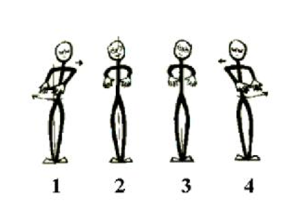
\includegraphics[height=5cm]{images/Exam_cli/Romberg.png}
    \caption{Illustration du test de Romberg}
    \label{fig:test_de_romberg}
\end{figure}


\begin{itemize}
    \item Le test de piétinement de Fukuda
\end{itemize}

Lors de ce test, le sujet doit reproduire un semblant de piétinement à raison d’un pas/seconde en levant le genou d’environ 45° et en maintenant les bras tendus vers l’avant. Il est invité à marcher sur place 50 fois, en levant les genoux bien hauts.
Afin d’obtenir de bon résultats, le test nécessite la mise en place de nombreuses précautions :  L'absence de sources sonores ou lumineuse, une élévation des cuisses à environ 45°, une fréquence approximative de 80 pas par minute, la position primaire des yeux à l'occlusion, la tête en position neutre puis tournée vers le côté droit puis gauche, si possible pieds nus, la mâchoires en position de posture mandibulaire après déglutition soit les dents qui ne se touchent pas.
Tout individu normal, piétinant sur place les yeux fermés, tourne sur lui-même seulement de 20° à 30° maximum en une cinquantaine de pas.

Ici, on peut observer :
\begin{itemize}
    \item 1.La tête tournée vers la gauche, l’individu dévie vers la droite.
    \item 2.La tête droite, un sujet normal lorsqu’il marque le temps, ne sort pas de la zone hachurée.
    \item 3.La tête tournée vers la droite, L’individu s’écarte vers la gauche.
\end{itemize}



\begin{figure}[H]
    \centering
    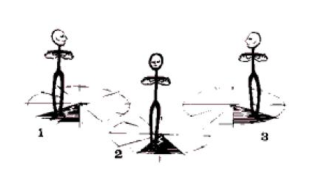
\includegraphics[height=5cm]{images/Exam_cli/pietinement.png}
    \caption{Illustration du test de piétinement de Fukuda} 
    \label{fig:test_de_Fukuda}
\end{figure}



\begin{itemize}
    \item Quelques alternatives :
    \begin{itemize}
        \item Test Unipodal 
        
        Ce test à pour objectif d’évaluer la stabilité statique du patient sur un seul appuie  afin d’identifier les individus présentant un faible équilibre, soit un risque accru de chute. Le but est de mettre en avant la proprioception  du patient et ainsi prouver l’intégrité fonctionnelle de son système postural. Le patient doit durant le test, se tenir sur une jambe, yeux ouverts, puis yeux fermés. Les paramètres stabilométriques mesurés via les oscillations permettent d’évaluer les capacités du patient à maintenir son équilibre.

\begin{figure}[H]
    \centering
    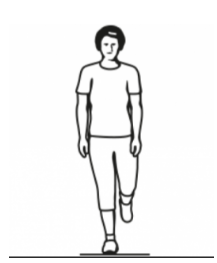
\includegraphics[height=5cm]{images/Exam_cli/Unipodal.png}
    \caption{Illustration du test Unipodal} 
    \label{fig:test_de_Unipodal}
\end{figure}
        
        \item   Test de la Perturbation Visuelle 
        Le test de la perturbation visuelle à pour but d’étudier la dépendance visuelle d’un sujet pour son équilibre. Le patient fixe alors un point visuel stable et un perturbation (changement du champ visuel, stimulation lumineuse) est introduite afin d'observer les compensations posturales de l’individu. 
    \end{itemize}
\end{itemize}

\newpage
\section{Annexe 2 : Méthodes d'analyse}
\label{annexe:2}

\subsection{Position moyenne du CdM}

\begin{equation}
  M_{AP} = \frac{1}{n} \sum_{n=1}^N \mbox{CdM}_{AP}(n) 
  \label{eq:M_AP}
\end{equation}

\begin{equation}
  M_{ML} = \frac{1}{n} \sum_{n=1}^N \mbox{CdM}_{ML}(n) 
  \label{eq:M_ML}
\end{equation}

La position moyenne du CdM représente la moyenne de l'ensemble des positions successives du CdM. 
Elle est calculée pour deux types de mouvements : les déplacements médio-latéraux ($M_{ml}$), ainsi que pour les déplacements antéro-postérieurs ($M_{ap}$).

Plus les valeurs sont basses, plus la qualité de l'équilibre est bonne.
La position moyenne est régulièrement couplée à l'écart-type, afin de pouvoir les situer l'un par rapport à l'autre, et ainsi donner une idée de la dispersion autour de la moyenne.

\subsection{Vitesse moyenne du CdM}

\begin{equation}
  L_{AP} = \sum_{n=1}^{N-1} \left| \mbox{CdM}_{AP}(n+1) - \mbox{CdM}_{AP}(n) \right|
  \label{eq:L_AP}
\end{equation}

\begin{equation}
  L_{ML} = \sum_{n=1}^{N-1} \left| \mbox{CdM}_{ML}(n+1) - \mbox{CdM}_{ML}(n) \right|
  \label{eq:L_ML}
\end{equation}

La mesure des longueurs des déplacements du centre de masse sur les deux axes (équations \ref{eq:L_AP} et \ref{eq:L_ML}) permettent d'estimer l'énergie dépensée pour la régulation de la posture orthostatique.

\begin{equation}
    MV_{AP} = \frac{L_{AP}}{T}
    \label{eq:MV_AP}
\end{equation}

\begin{equation}
    MV_{AP} = \frac{L_{ML}}{T}  
    \label{eq:MV_ML}    
\end{equation}

Les vitesses ainsi calculées représentent alors le tracé total en fonction du temps. 
Une vitesse élevée signifie un mauvais équilibre. 
Elles peuvent aussi renseigner sur la consommation d'énergie.

\subsection{Valeur quadratique moyenne (RMS pour root mean square)}

\begin{equation}
    RMS_{AP} =\sqrt{  \frac{\sum_{n=1}^{N} \left (\text{CoM}_{AP}(n) \right)^2 }{N}}
    \label{eq:RMS_AP}
\end{equation}

\begin{equation}
    RMS_{ML} =\sqrt{  \frac{\sum_{n=1}^{N} \left (\text{CoM}_{ML}(n) \right)^2 }{N}}
    \label{eq:RMS_ML}
\end{equation}

Le calcul des moyennes quadratiques des amplitudes de déplacement du CdM sur les deux axes définis précédemment permet de quantifier l'habileté à maintenir l'équilibre. 
Plus ces mesures sont basses, plus l'habileté est grande.

\subsection{Écart maximal}

\begin{equation}
  R_{AP}= max \left ( \text CoM_{AP} \right ) - min\left ( \text CoM_{AP} \right ) 
  \label{eq:R_AP}
\end{equation}

\begin{equation}
  R_{ML}= max \left ( \text CoM_{ML} \right ) - min\left ( \text CoM_{ML} \right )   
  \label{eq:R_ML}
\end{equation}


L'écart maximal est la différence entre la position maximale et minimale du CdM et est défini suivant les deux axes AP et ML.
Une augmentation d'une de ces valeurs peut être interprétable en une baisse de la capacité à maintenir l'équilibre postural.

\subsection{Surface de l'ellipse de confiance (CEA)}

\begin{equation}
CEA= 6\pi \sqrt{ \left ( \frac{\sum_{n=1}^{N} \left (\text{CoM}_{AP}(n) \right)^2 \times \sum_{n=1}^{N} \left ( \text{CoM}_{ML}(n) \right)^2}{N^2} \right ) - \left (\frac{\sum_{n=1}^N \text{CoM}_{AP} \times CoM_{ML}}{N} \right)^2}
\label{eq:CEA}
\end{equation}

La surface de l'ellipse de confiance regroupe un certain pourcentage du statokinésigramme (en cm2), ici 95\%. 
Cette intervalle de confiance peut varier selon les pratiques ou les habitudes (certains praticiens utilisent une surface d'ellipse de confiance de 90\% par exemple). 
Plus précisément, c'est l'évolution du périmètre de l'ellipse qui est étudiée. 
Plus ce périmètre est grand, et plus l'équilibre est mauvais.

\begin{figure}[H]
    \centering
    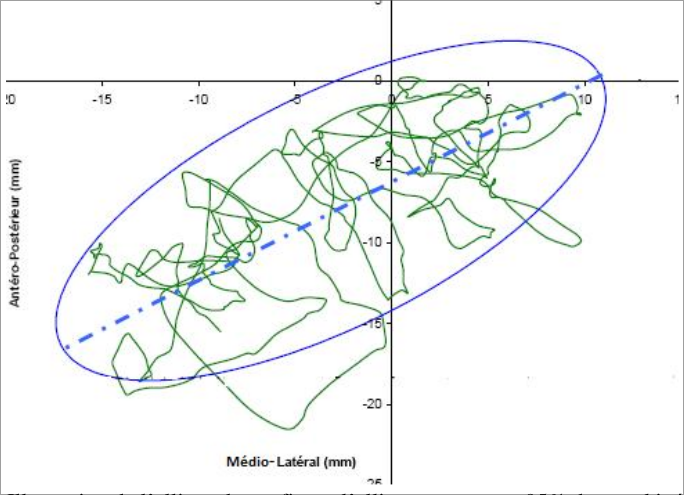
\includegraphics[height=8cm]{images/methode/ellipse_confiance_95.png}
    \caption{Illustration de l'ellipse de confiance (à 95\% du statokinésigramme)}\label{fig:ellipse_confiance}
\end{figure}

\subsection{Quotient de Romberg}

\begin{equation}
  QR = \frac{\text{CEA}_{\text{YF}}}{\text{CEA}_{\text{YO}}}
  \label{eq:QR}
\end{equation}

Ce quotient entre la valeur de CEA yeux fermés et la valeur de CEA yeux ouverts permet de mettre en évidence le rôle de la vision dans le contrôle de la posture. 
Une valeur élevée de ce quotient indique une dépendance visuelle accrue dans le maintien de l'équilibre.

\subsection{Fréquence moyenne ou centroïdale}

\begin{equation}
  \text{FM}_{\text{AP}} = \frac{\text{MV}_{\text{AP}}}{4\cdot\sqrt{2}\cdot\text{M}_{\text{AP}}}
  \label{eq:FM_AP}
\end{equation}

\begin{equation}
  \text{FM}_{\text{ML}} = \frac{\text{MV}_{\text{ML}}}{4 \cdot \sqrt{2} \cdot \text{M}_{\text{ML}}}
  \label{eq:FM_ML}
\end{equation}

La fréquence moyenne est le paramètre qui permet d'étudier le temps nécessaire au mouvement analysé pour revenir dans une position identique. 
Son calcul passe par l'analyse de la distribution fréquentielle des amplitudes.

\subsection{périodogramme}
\label{subsubsec:periodogramme}

Réaliser un périodogramme est l'une des méthodes les plus simples pour estimer la \textbf{densité spectrale de puissance} d'un signal (ici posturographique).
Cette méthode se base sur la transformée de Fourier discrète (échantillonnée) du signal.
Plus précisément, le périodogramme est le carré du module de la TFD normalisée par la longueur du signal.

\begin{equation}
  P_{\text{Per}}(f)=\frac{1}{NT_e}\left|\sum\limits_{n=0}^{N-1}x(nT_e)e^{-j2\pi nT_ef}\right|^2
  \label{eq:P_per}
\end{equation}

\begin{figure}[ht]
  \centering
  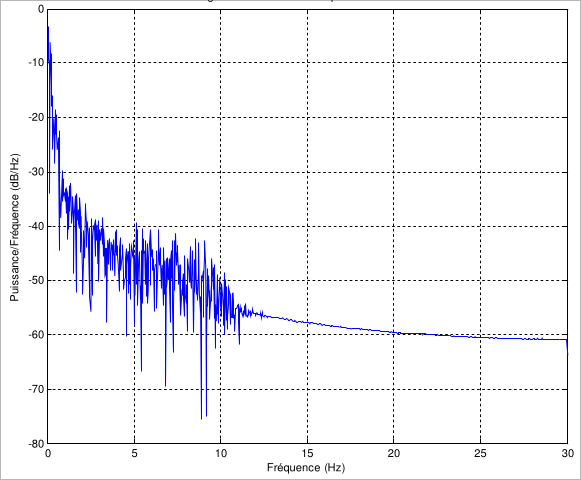
\includegraphics[width=8cm]{images/methode/periodogramme.png}
  \caption{Illustration d'un périodogramme d'un signal posturographique}
  \label{fig:periodogramme}
\end{figure}

On peut observer sur la figure \ref{fig:periodogramme} la répartition de l'énergie par fréquence.
Concrètement, de l'énergie dans les fréquences basses correspond à des ajustements lents, montrant une bonne stabilité contrairement à si on en avait trouvé dans les hautes fréquences.

\subsection{Estimateur de Welch}

L'estimateur de Welch est une amélioration apportée au périodogramme.
Cette méthode permet d'augmenter la qualité de l'estimation de la densité spectrale de puissance.
Cette méthode passe par le moyennage de $L$ périodogrammes partiels.
Un périodogramme partiel est simplement le périodogramme estimé d'un \textbf{segment du signal} (longueur du segment notée $l$).
Chaque segment du signal est fenêtré afin de réduire les effets de bord (distortions) qui peuvent apparaître lors de la TFD.

\begin{equation}
  P_{\text{Welch}}(f)=\frac{1}{L}\sum\limits_{l=1}^{L-1}P_l(f)
  \label{eq:P_Welch}
\end{equation}

\begin{equation} 
  P_l(f) = \frac{1}{K}\left|\sum\limits_{n=0}^{K-1}x(n+lK)\omega(n)e^{-j2\pi nf}\right|^2
  \label{eq:P_l}
\end{equation}

$P_l(f)$ est le périodogramme de chaque segment (on utilise la formule \ref{eq:P_per}).

\begin{figure}[ht]
  \centering
  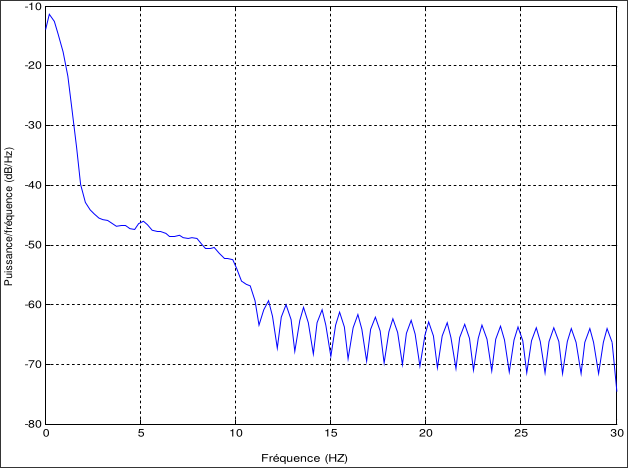
\includegraphics[width=8cm]{images/methode/welch.png}
  \caption{Illustration de la densité spectrale par estimateur de Welch}
  \label{fig:welch}
\end{figure}

La figure \ref{fig:welch} montrant les valeurs estimées par calcul de l'estimateur de Welch se base sur les mêmes données médicales que la figure \ref{fig:periodogramme}.

\subsection{Analyse de la pente du spectre de puissance et régression}
\label{subsubsec:pente}

L’analyse du spectre dans le plan log-log permet de mieux comprendre les mécanismes de régulation posturale et de quantifier la stabilité ou l’instabilité en fonction des fréquences des oscillations du CdM ou CdP. 
La régression linéaire dans ce contexte permet d’estimer la pente du spectre et de révéler les caractéristiques de contrôle postural.

% TODO : make welch and periodogram on the same figure

\begin{figure}[ht]
    \centering
    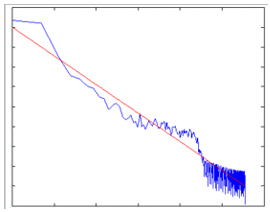
\includegraphics[height=5cm]{images/methode/analyse_spec_regre_lin.png}
    \caption{Analyse spectrale et régression linéaire}\label{fig:regression_lineaire}
\end{figure}

Lorsque la pente est fortement négative, (par convention aux alentours de $-2$ ou plus), cela signifie que les oscillations posturales à basse fréquences dominent, ce qui peut souligner un contrôle postural efficace.

Lorsque la pente est moins négative, (aux alentours de $-1$), cela montre que les oscillations à hautes fréquences contribuent beaucoup plus au maintien de la stabilité.
Il est possible d'en déduire un mauvais contrôle postural, souvent observé chez les personnes agées.

\newpage
\section{Annexe 3 : prototype complet}

\begin{figure}[H]
    \centering
    \caption{Plateforme imaginée}
    \begin{minipage}{0.3\textwidth}
        \centering
        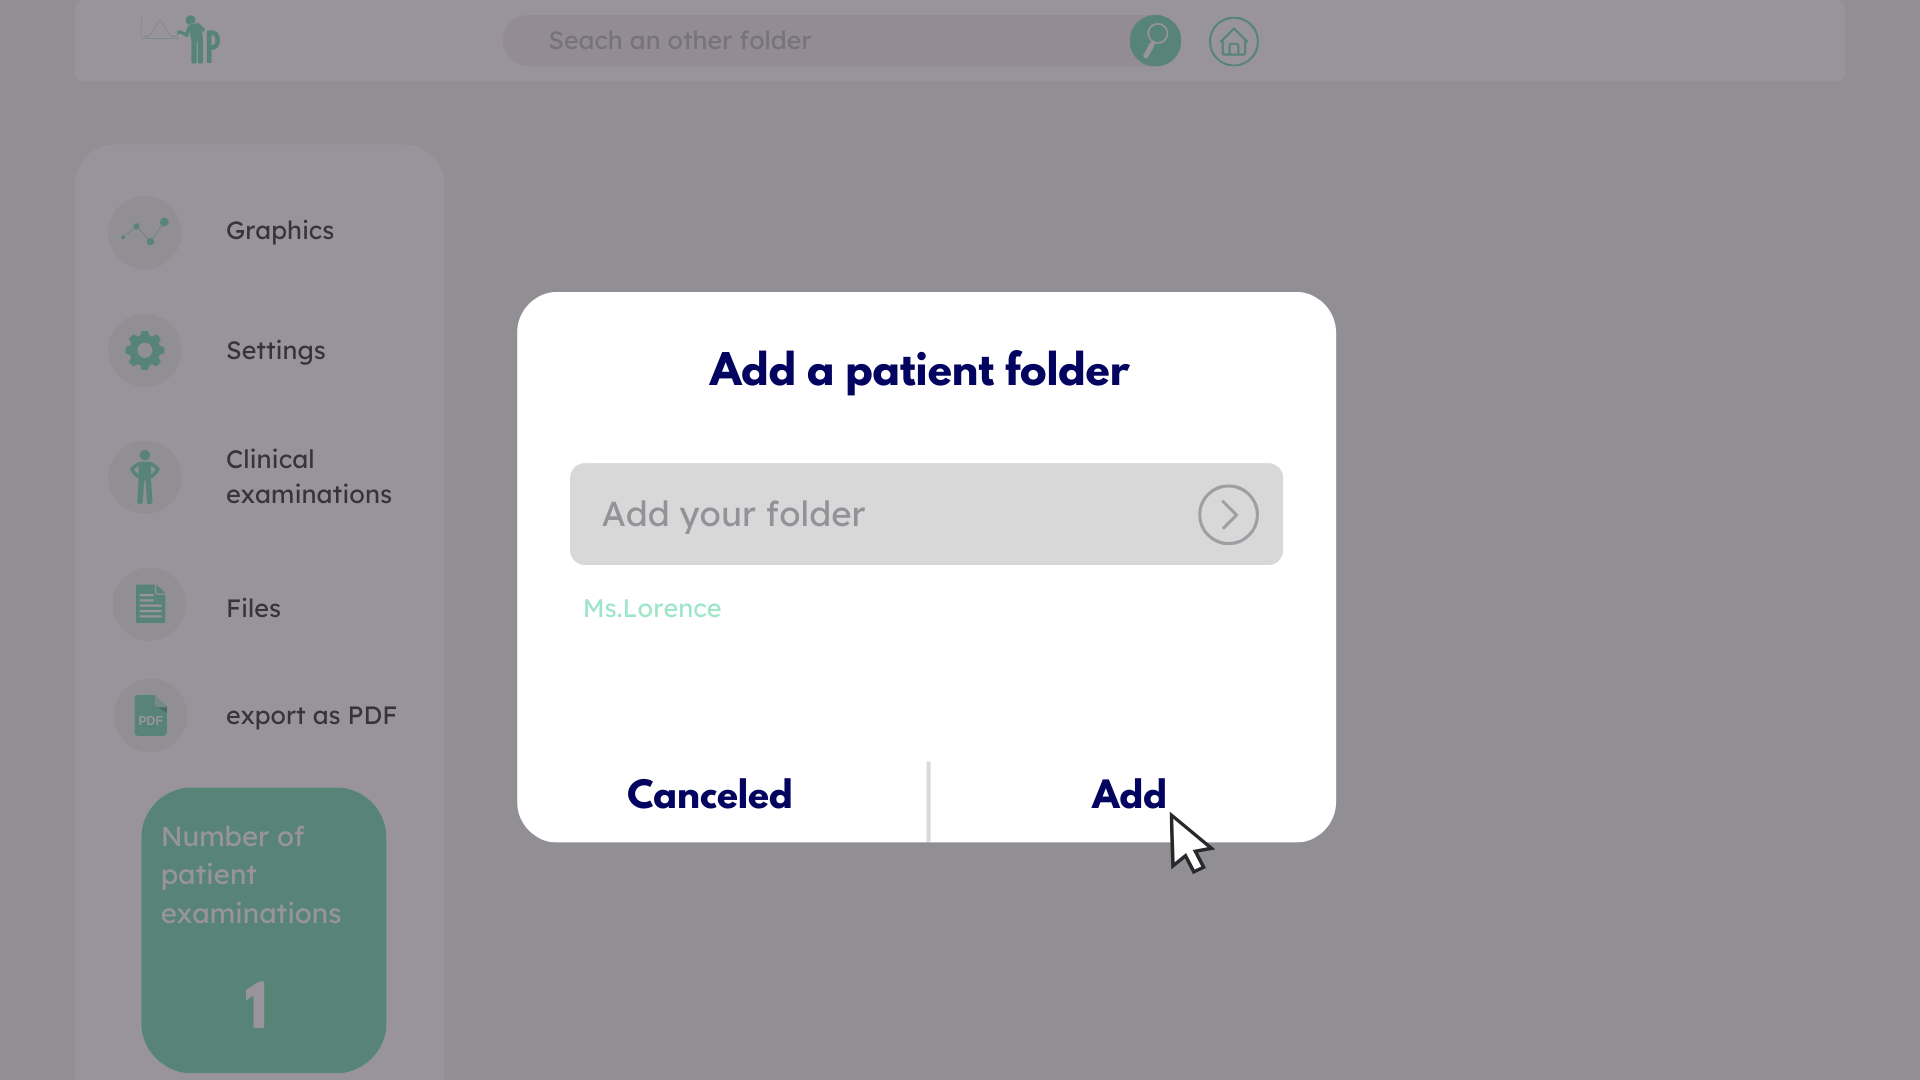
\includegraphics[width=\textwidth]{images/Prototype/1.png}
        \caption*{1}
    \end{minipage}
    \begin{minipage}{0.3\textwidth}
        \centering
        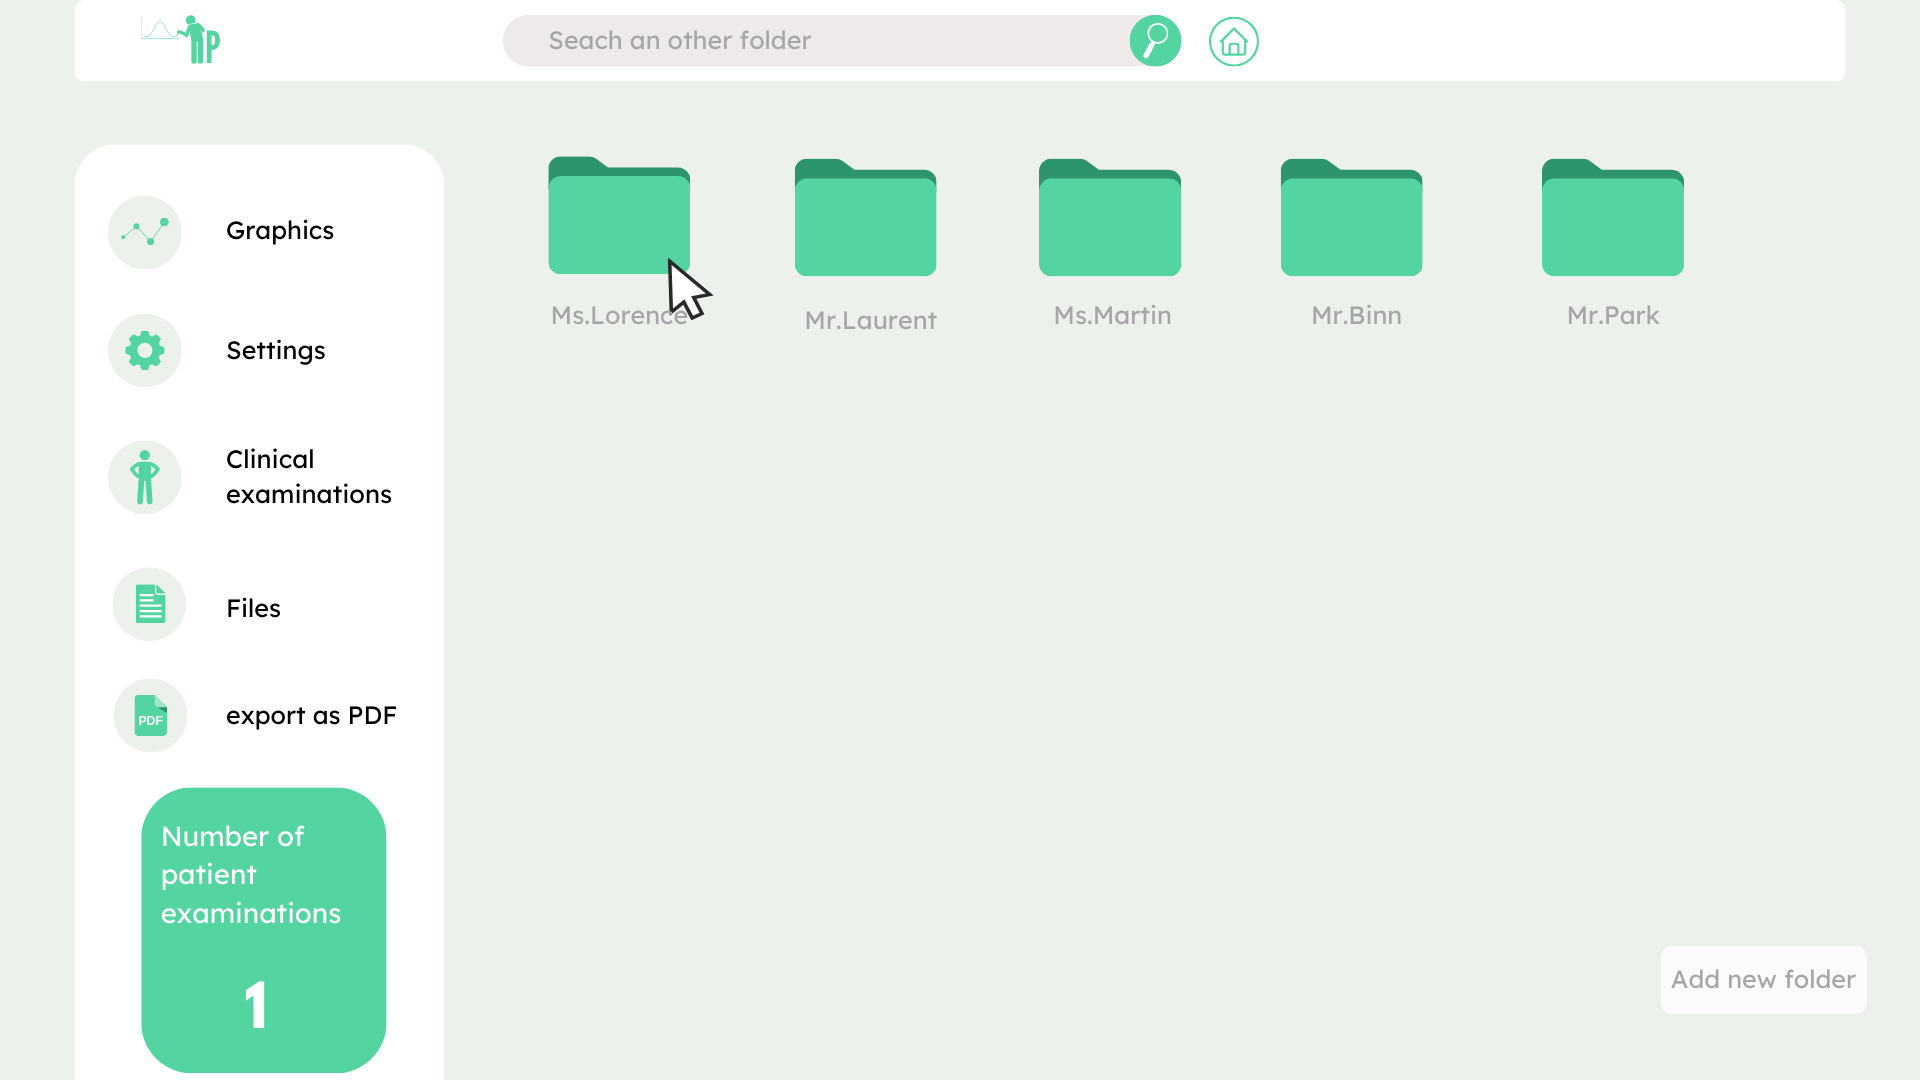
\includegraphics[width=\textwidth]{images/Prototype/Accueil de la plateforme de visualisation.png}
        \caption*{2}
    \end{minipage}
    \begin{minipage}{0.3\textwidth}
        \centering
        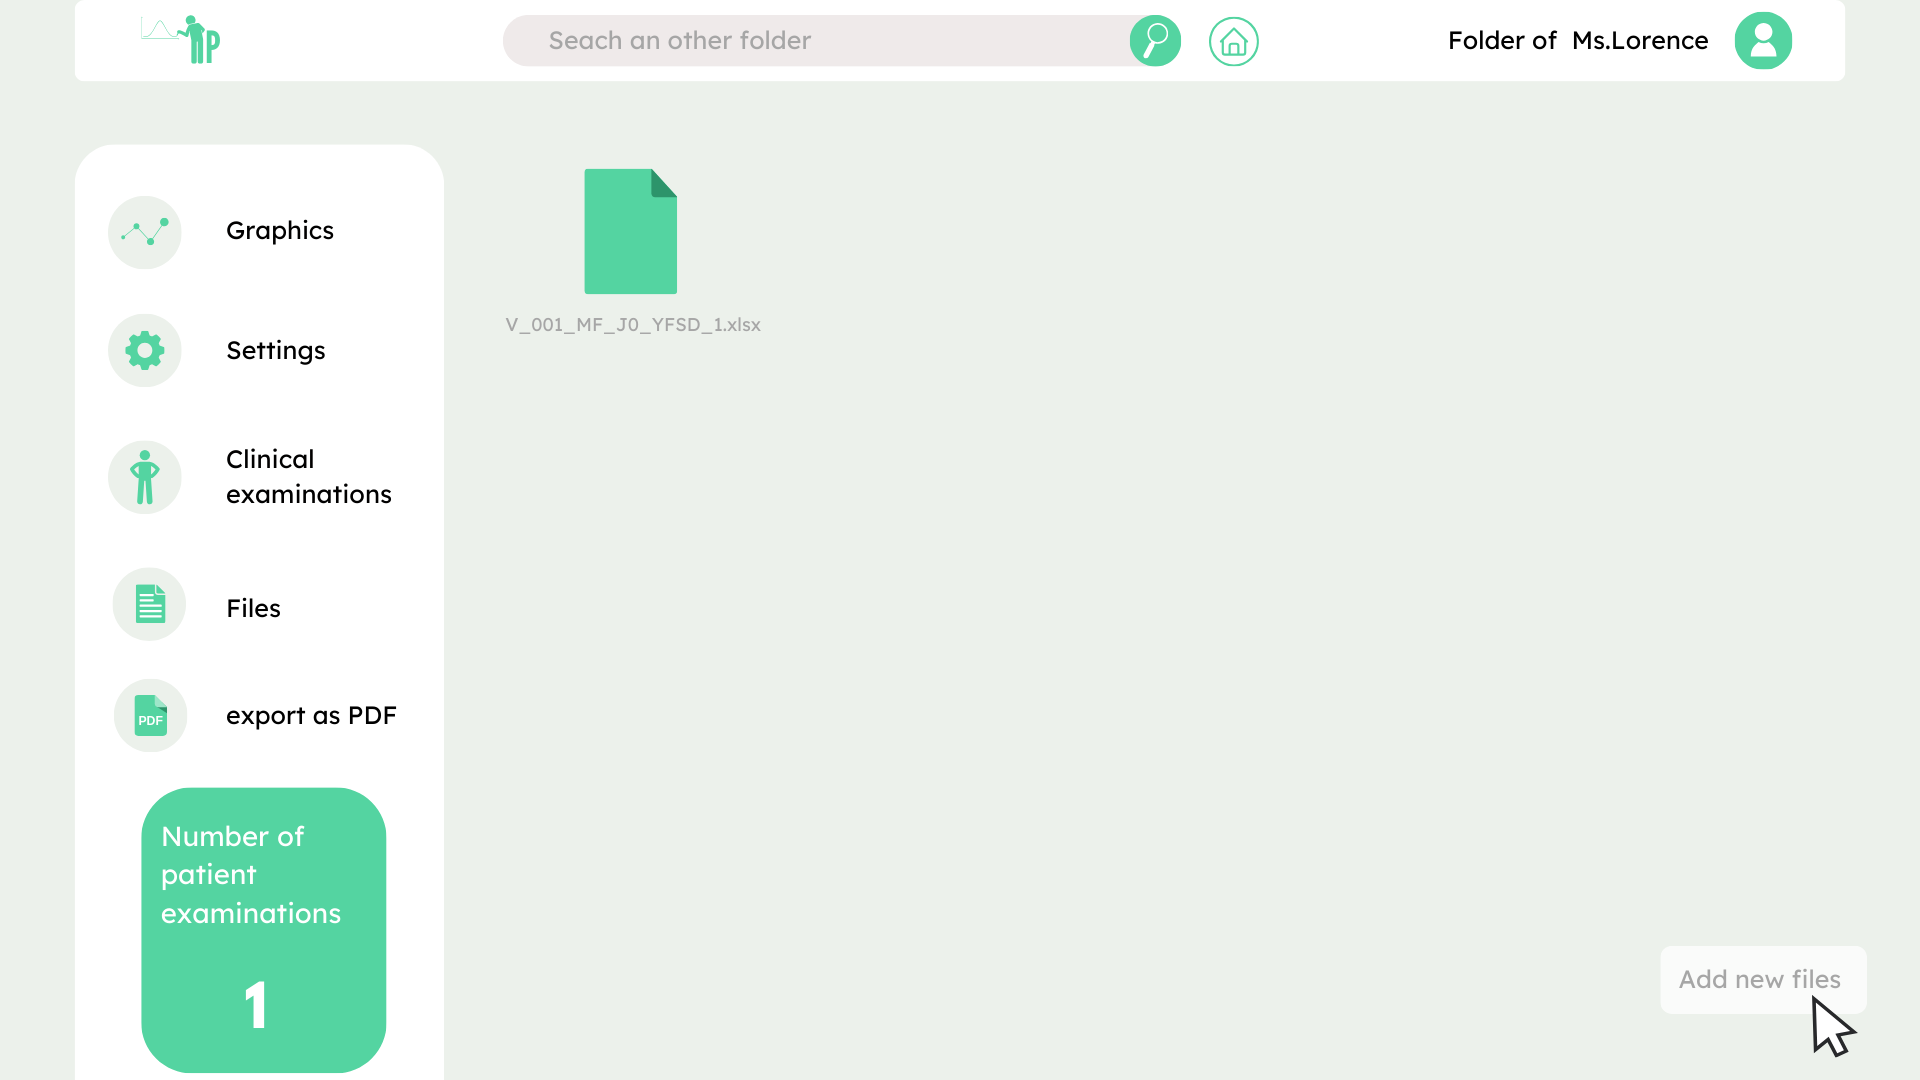
\includegraphics[width=\textwidth]{images/Prototype/3.png}
        \caption*{3}
    \end{minipage}
    \begin{minipage}{0.3\textwidth}
        \centering
        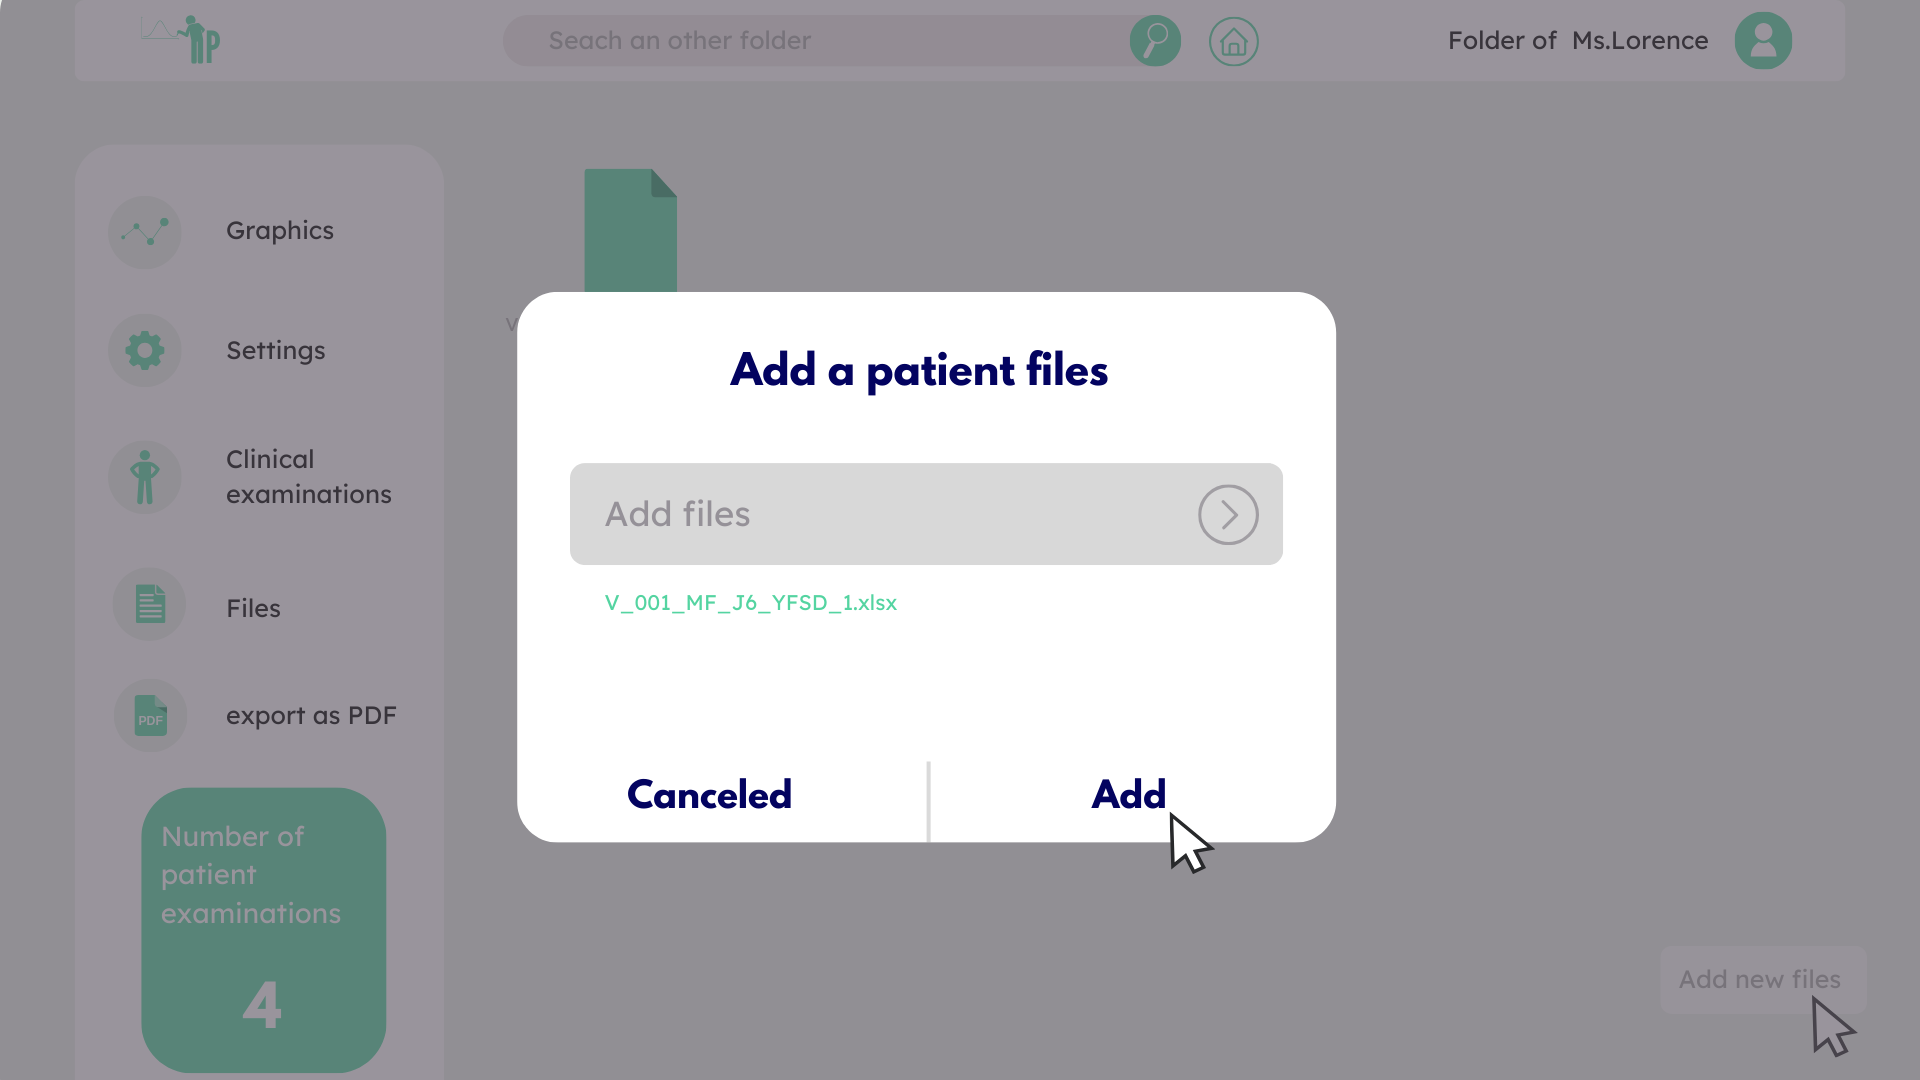
\includegraphics[width=\textwidth]{images/Prototype/4.png}
        \caption*{4}
    \end{minipage}
    \begin{minipage}{0.3\textwidth}
        \centering
        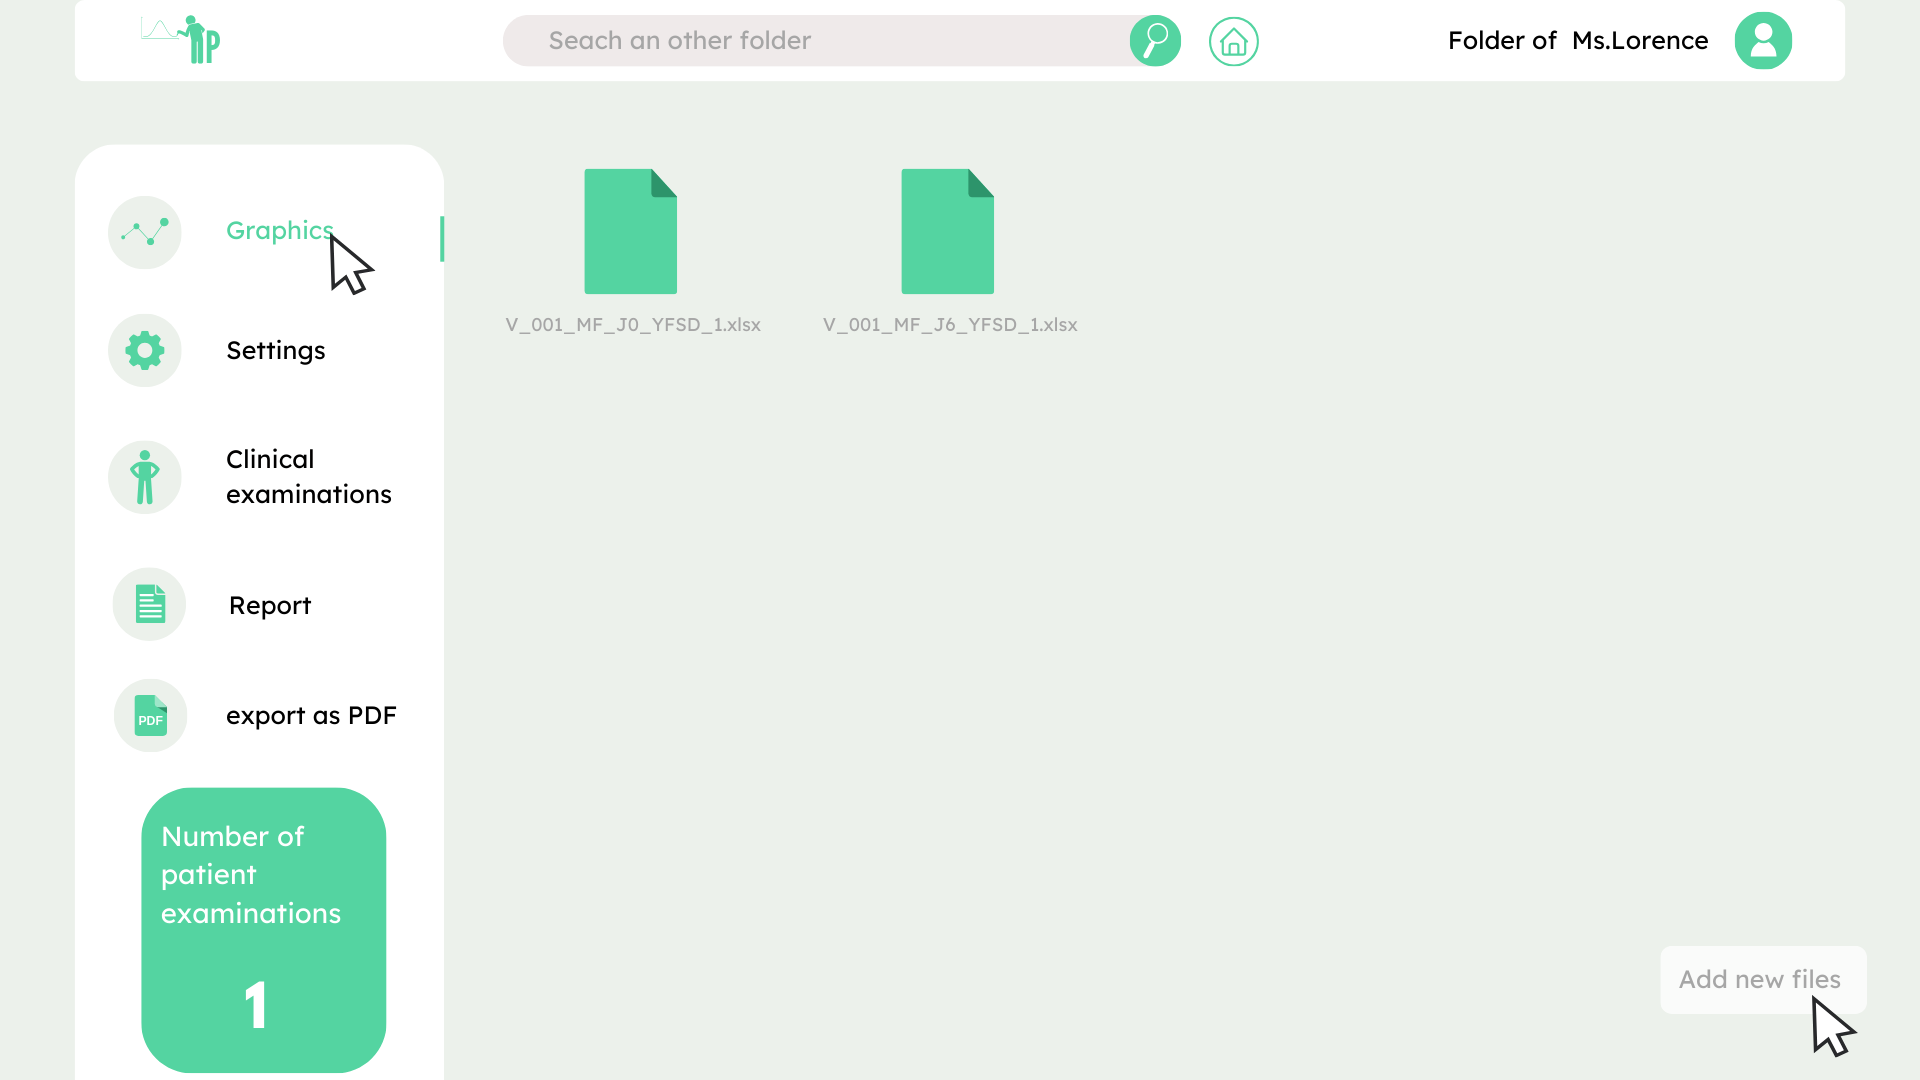
\includegraphics[width=\textwidth]{images/Prototype/5.png}
        \caption*{5}
    \end{minipage}
    \begin{minipage}{0.3\textwidth}
        \centering
        
\includegraphics[width=\textwidth]{images/Prototype/6.png}
        \caption*{6}
    \end{minipage}
    \begin{minipage}{0.3\textwidth}
        \centering
        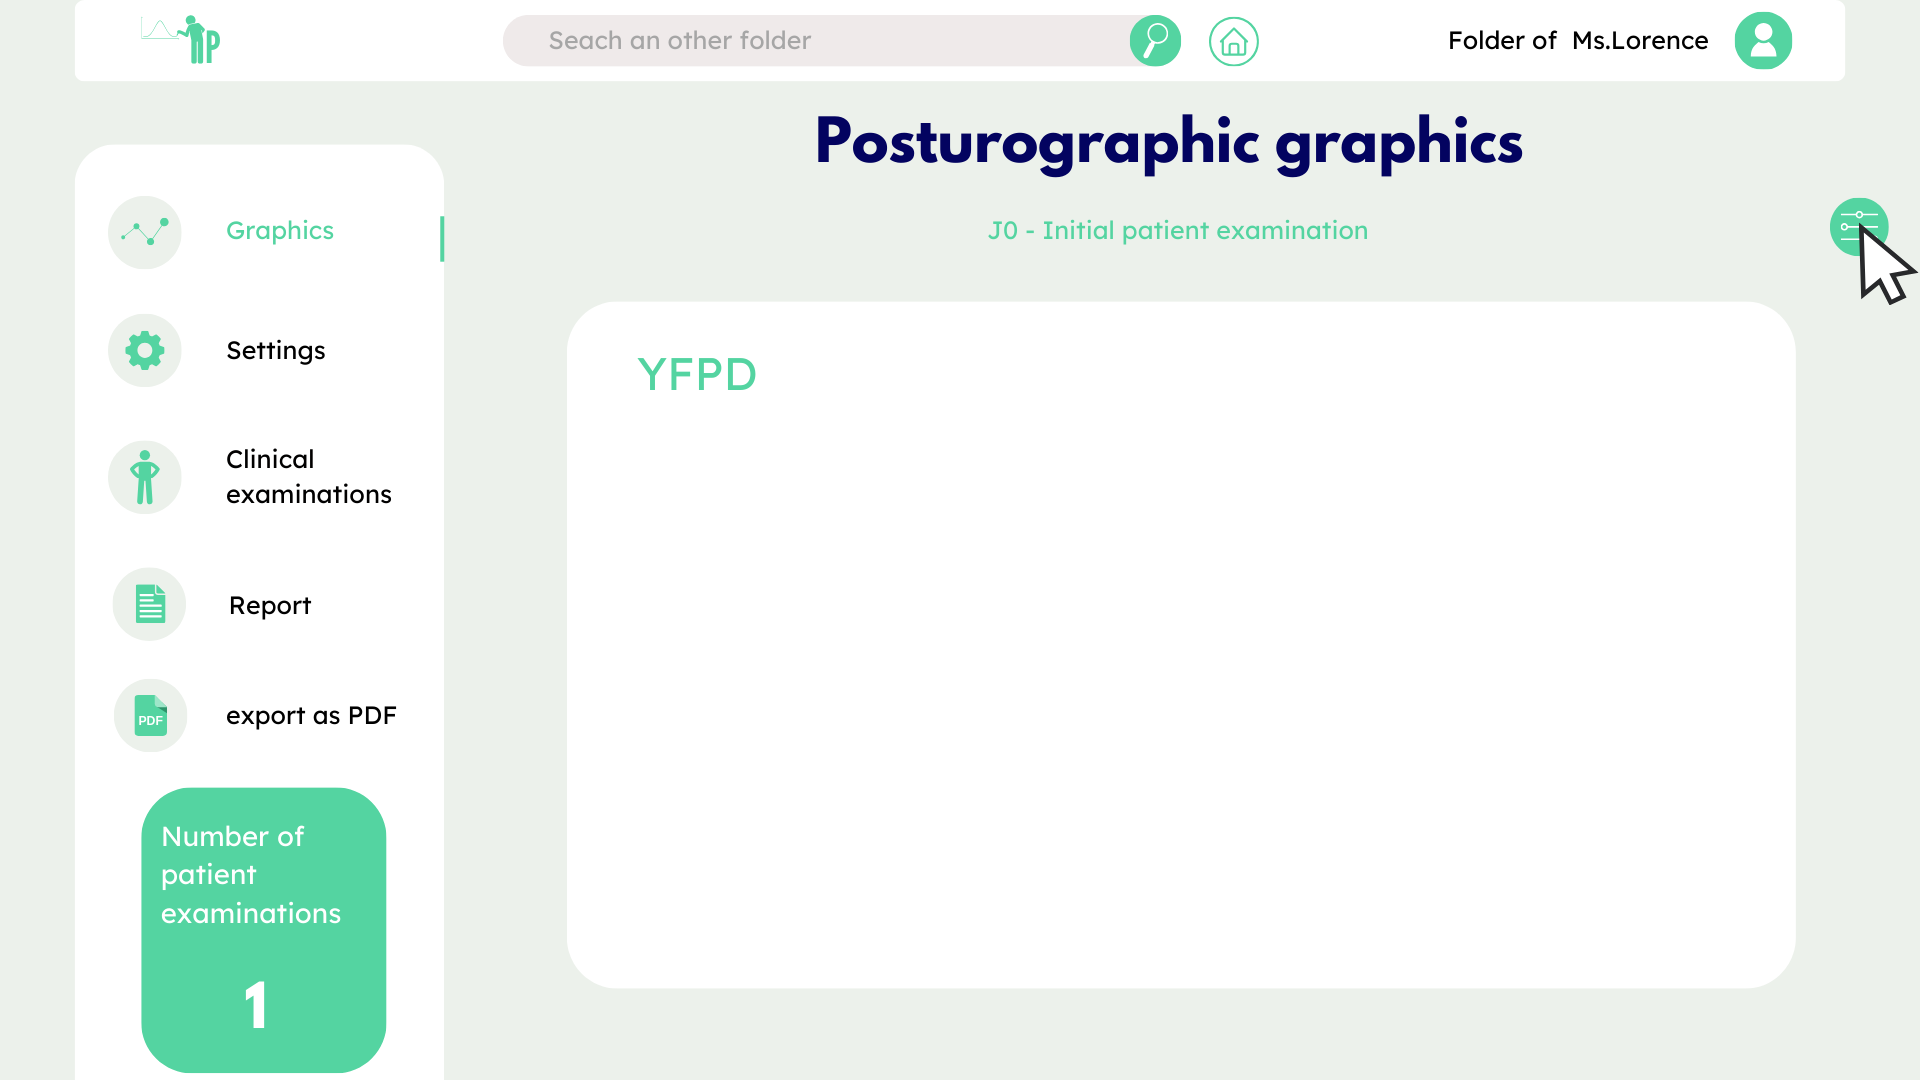
\includegraphics[width=\textwidth]{images/Prototype/7.png}
        \caption*{7}
    \end{minipage}
    \begin{minipage}{0.3\textwidth}
        \centering
        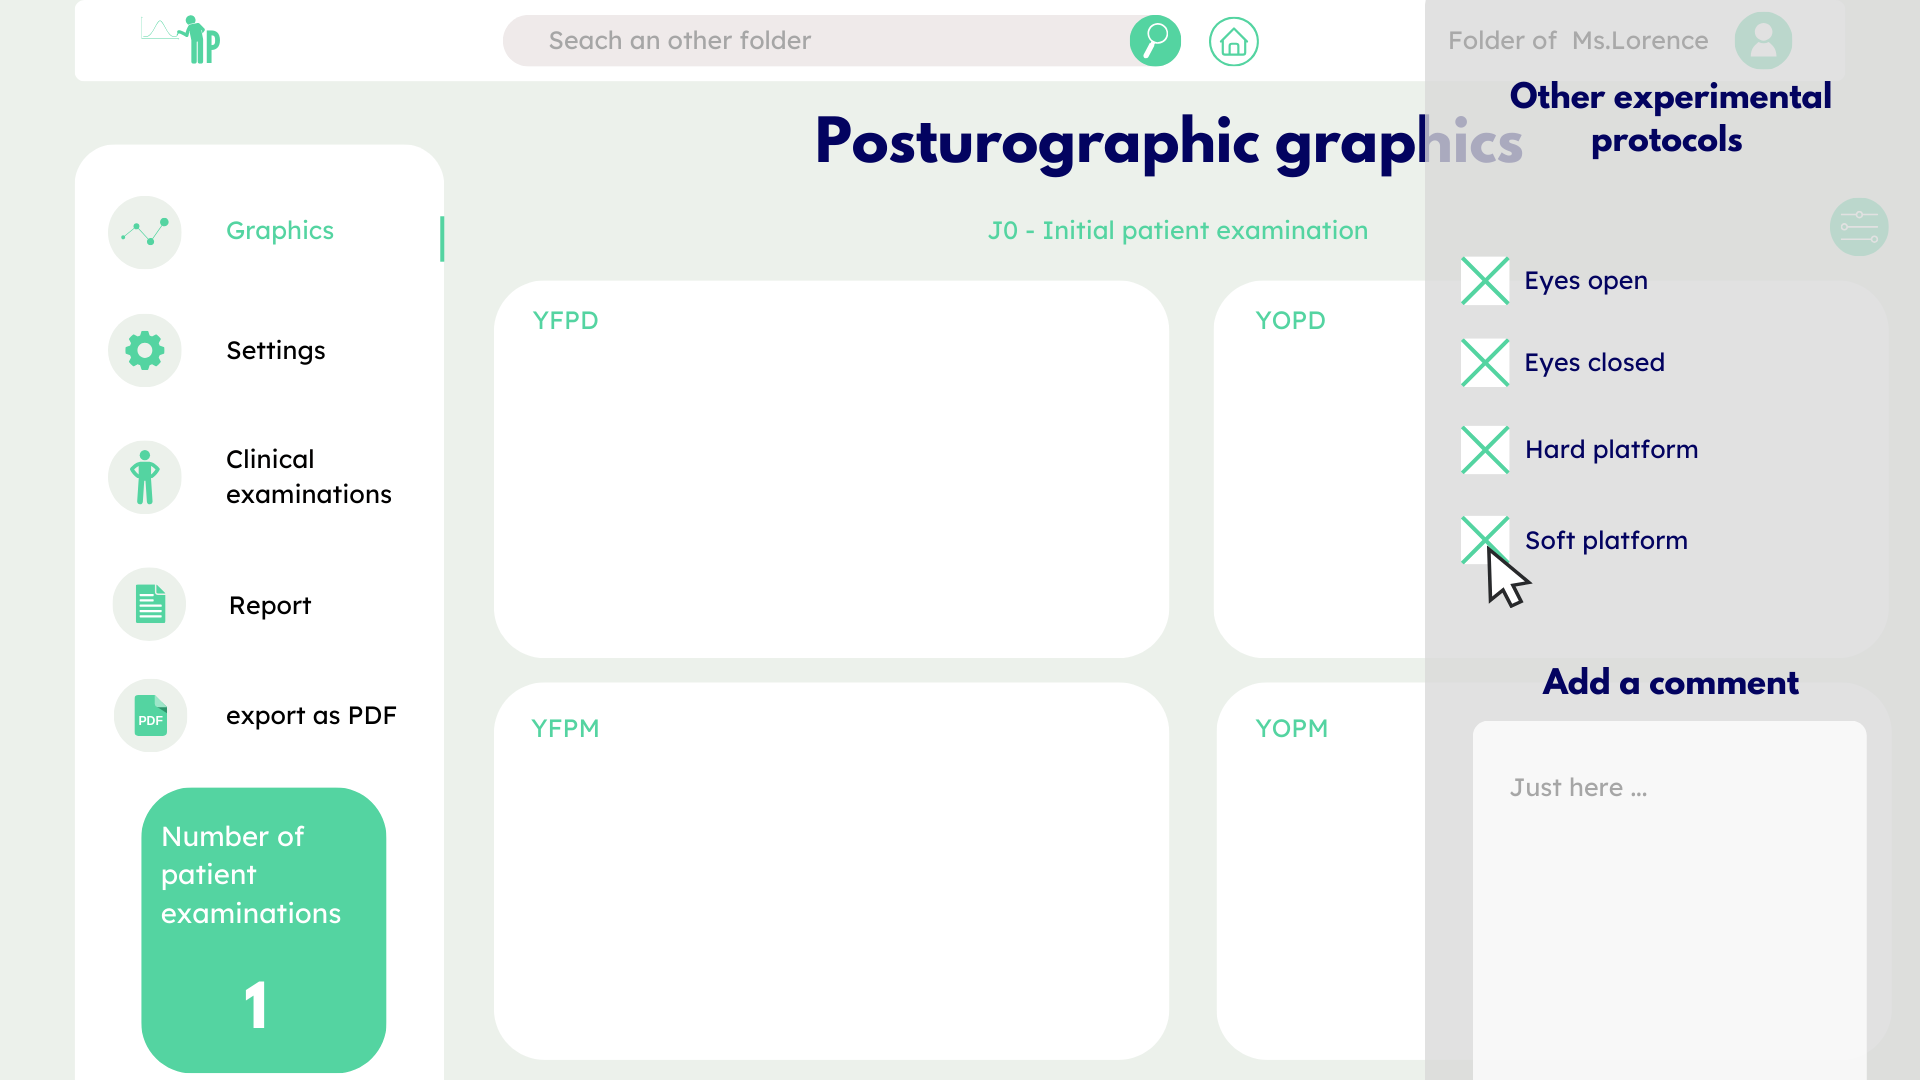
\includegraphics[width=\textwidth]{images/Prototype/Visualisation des données en fonction de différents protocoles expérimentaux.png}
        \caption*{8}
    \end{minipage}
    \begin{minipage}{0.3\textwidth}
        \centering
        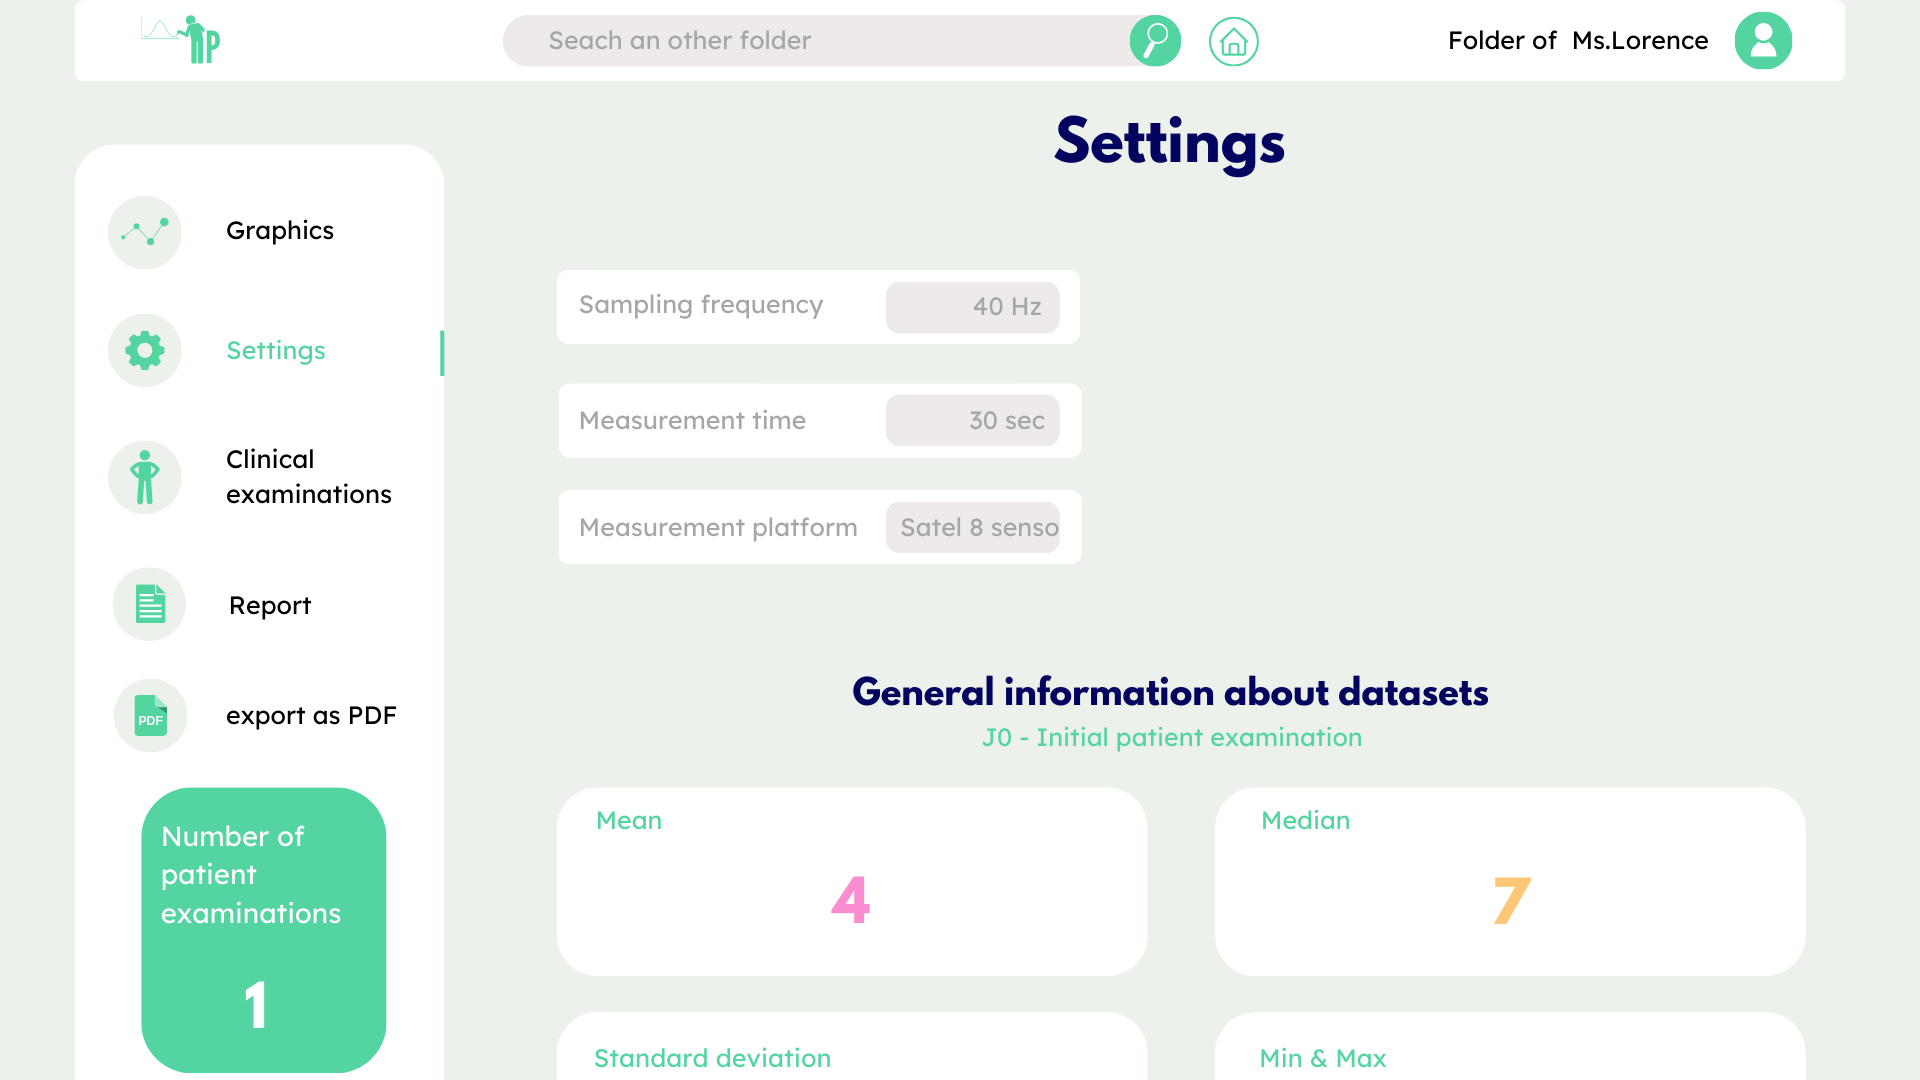
\includegraphics[width=\textwidth]{images/Prototype/visualiser des données clés du jeu de données étudié.png}
        \caption*{9}
    \end{minipage}
    \begin{minipage}{0.3\textwidth}
        \centering
        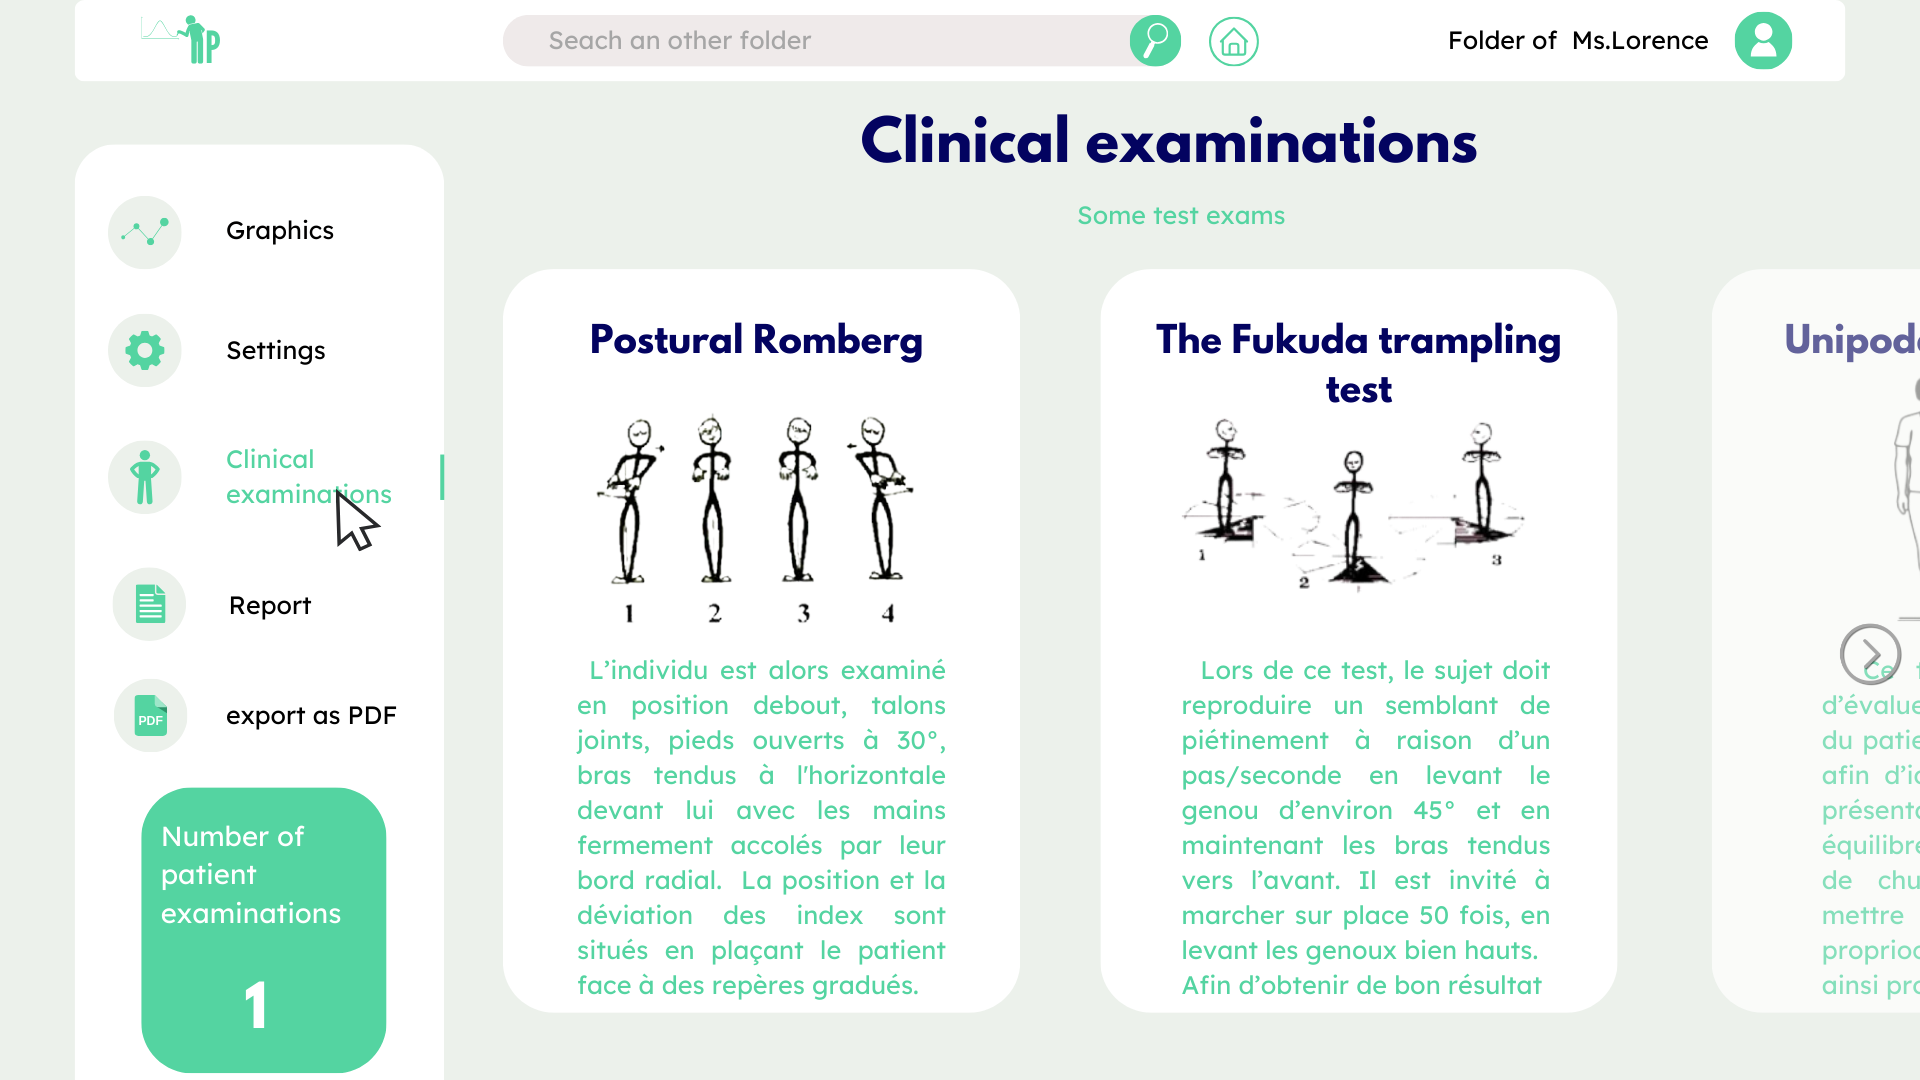
\includegraphics[width=\textwidth]{images/Prototype/10.png}
        \caption*{10}
    \end{minipage}
    \begin{minipage}{0.3\textwidth}
        \centering
        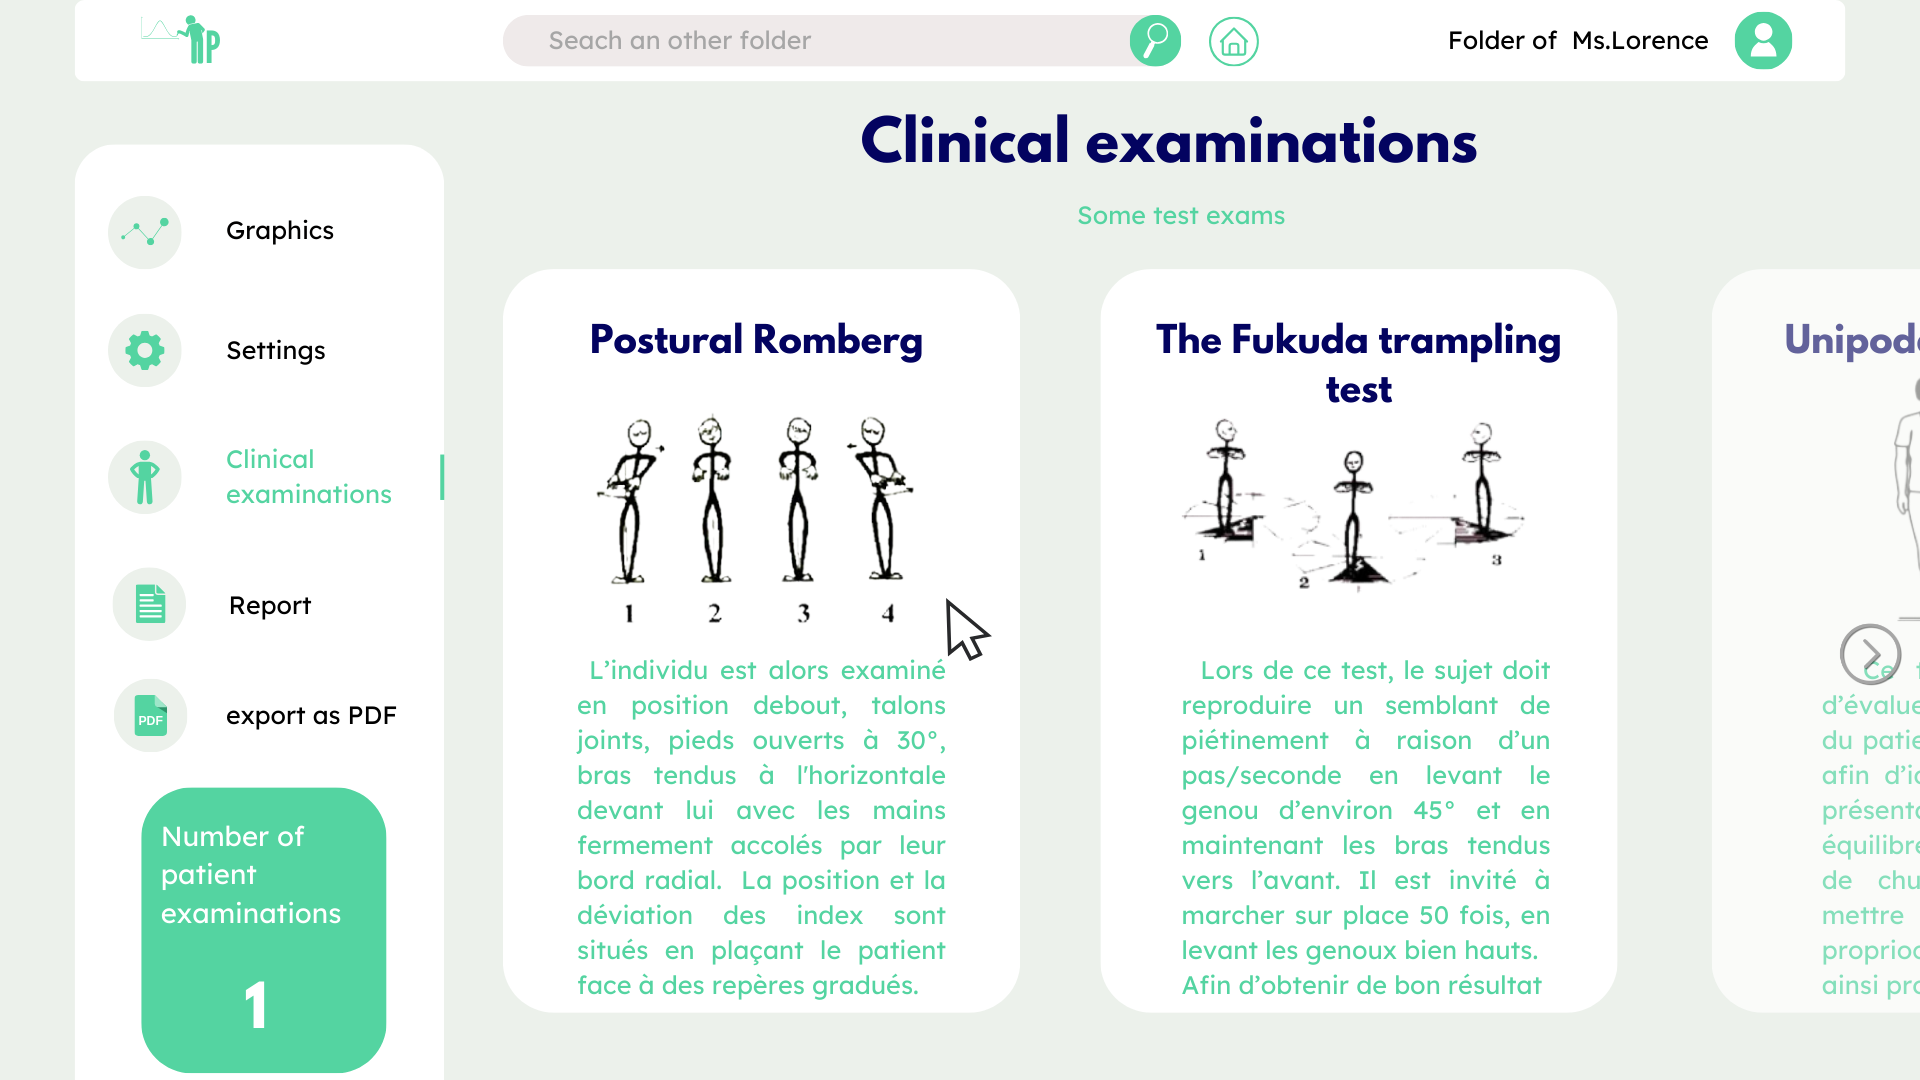
\includegraphics[width=\textwidth]{images/Prototype/11.png}
        \caption*{11}
    \end{minipage}
    \begin{minipage}{0.3\textwidth}
        \centering
        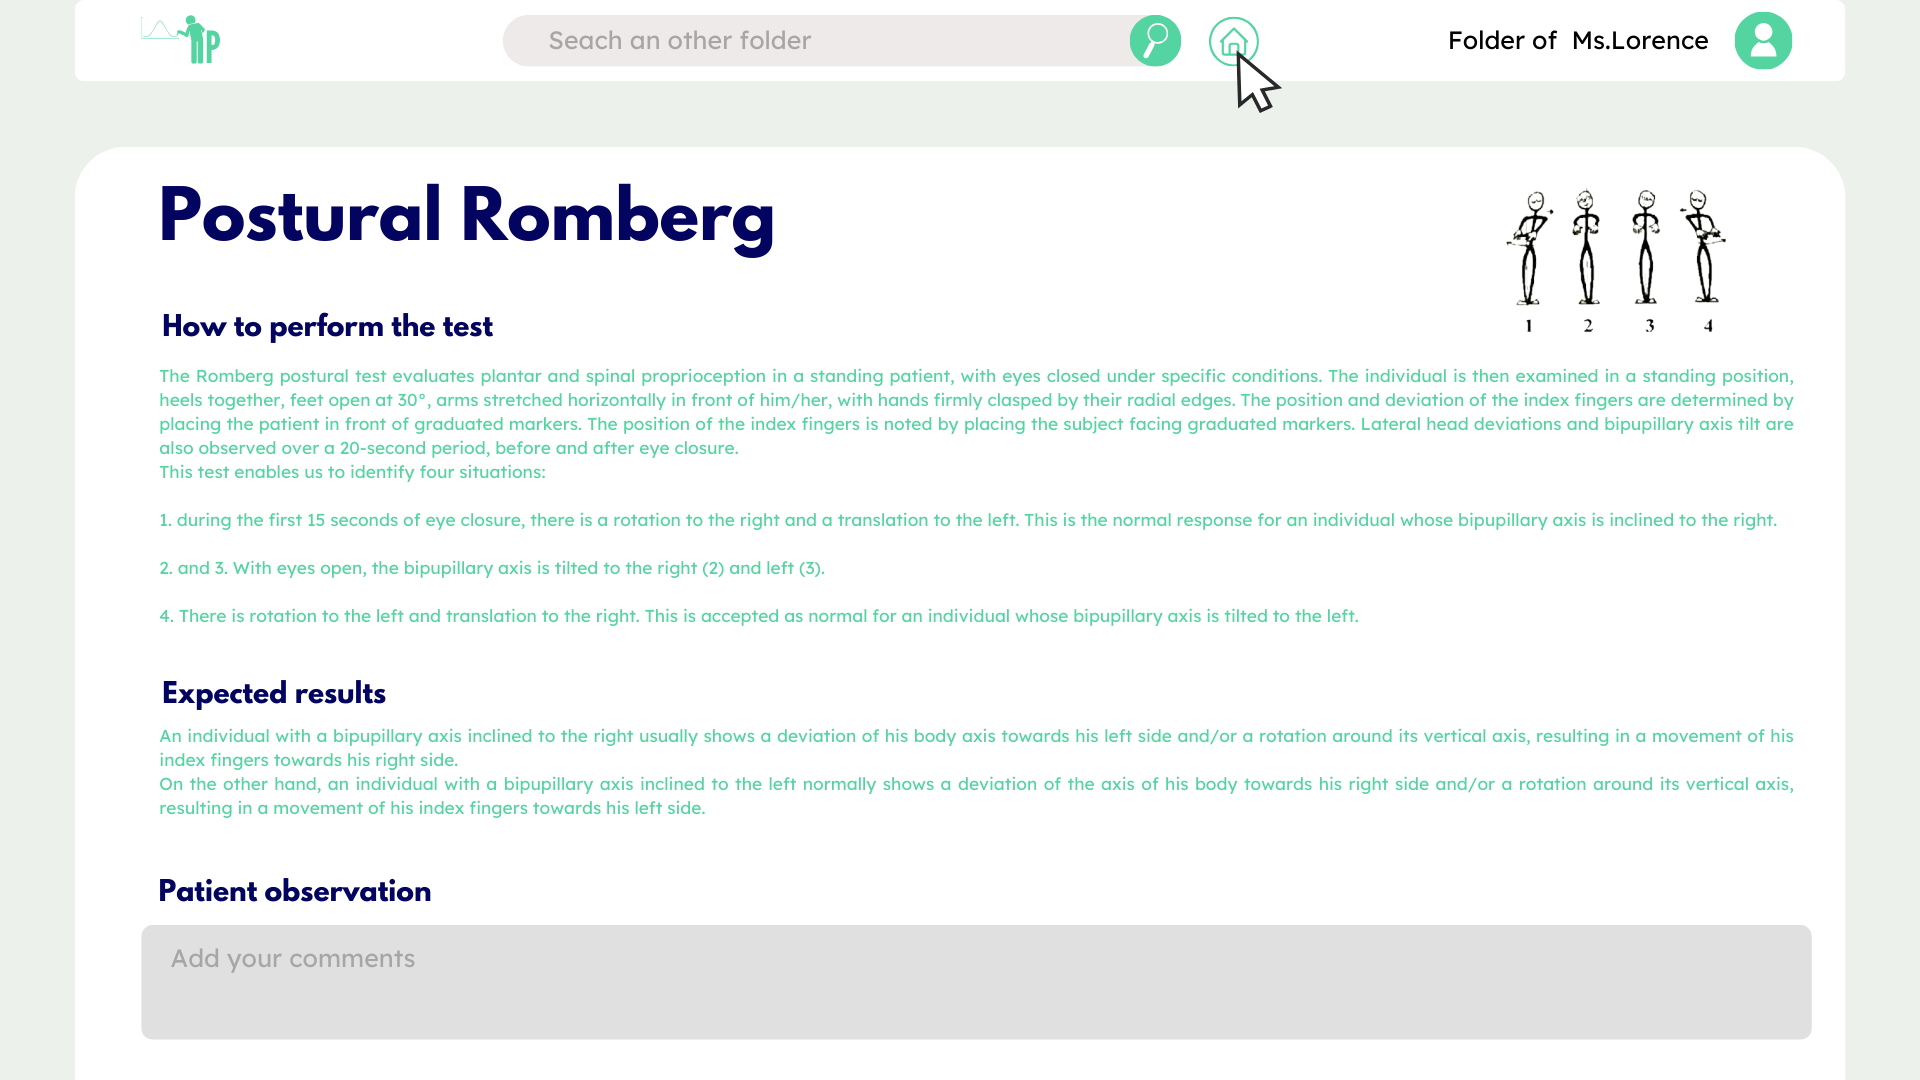
\includegraphics[width=\textwidth]{images/Prototype/12.png}
        \caption*{12}
    \end{minipage}
    \begin{minipage}{0.3\textwidth}
        \centering
        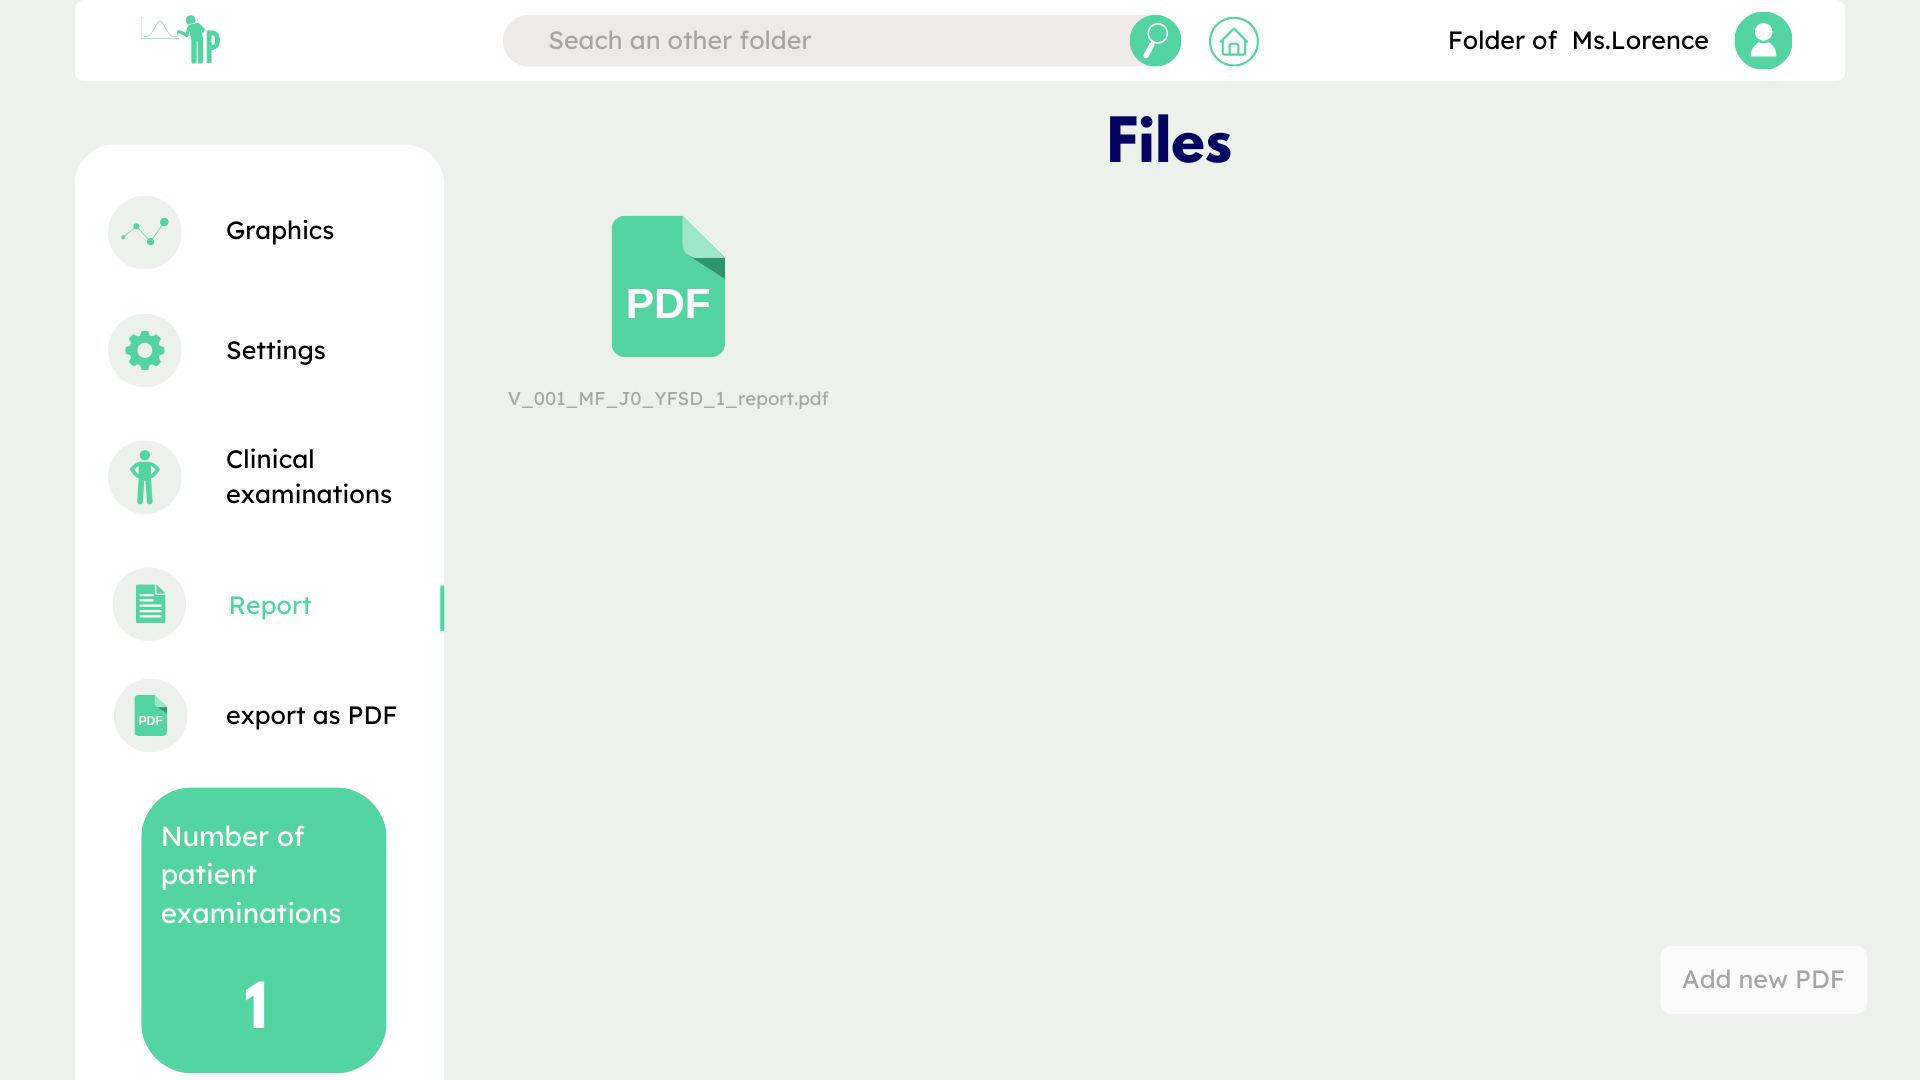
\includegraphics[width=\textwidth]{images/Prototype/13.png}
        \caption*{13}
    \end{minipage}
    \begin{minipage}{0.3\textwidth}
        \centering
        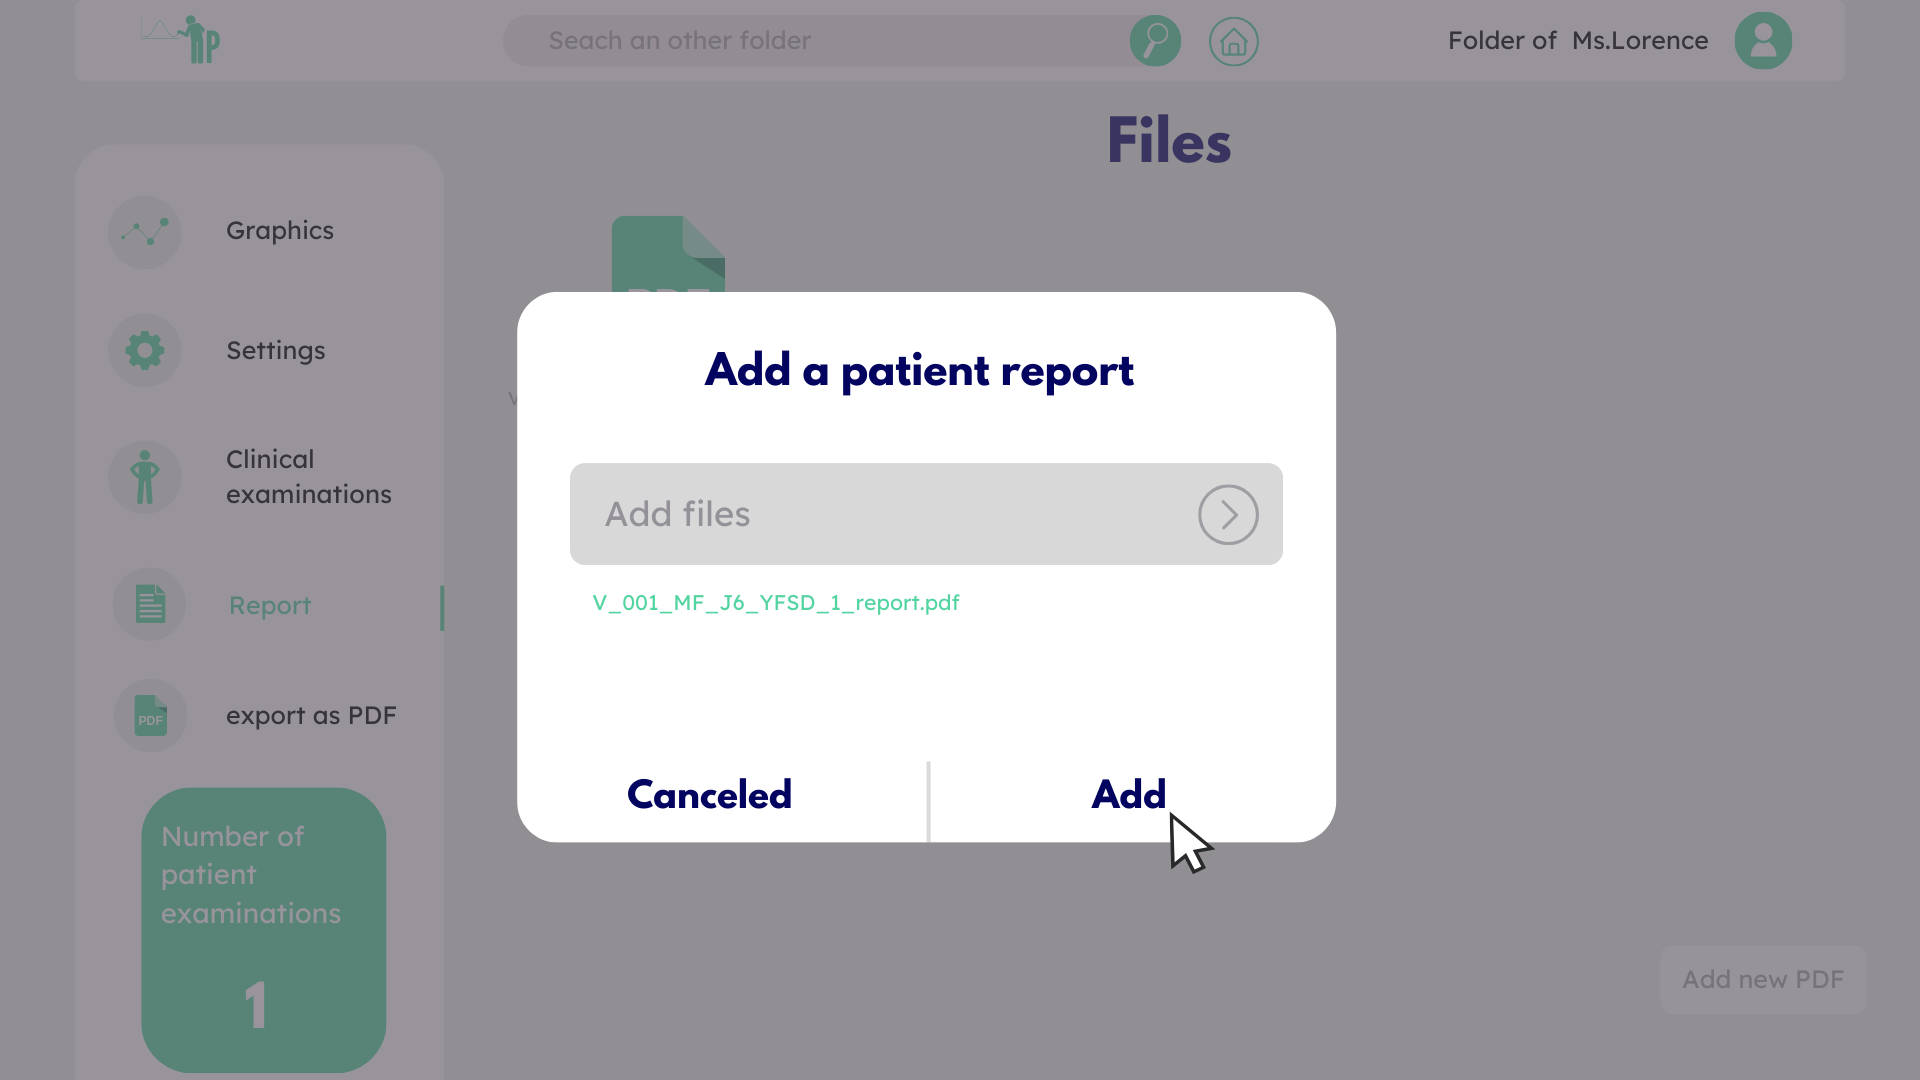
\includegraphics[width=\textwidth]{images/Prototype/14.png}
        \caption*{14}
    \end{minipage}
    \begin{minipage}{0.3\textwidth}
        \centering
        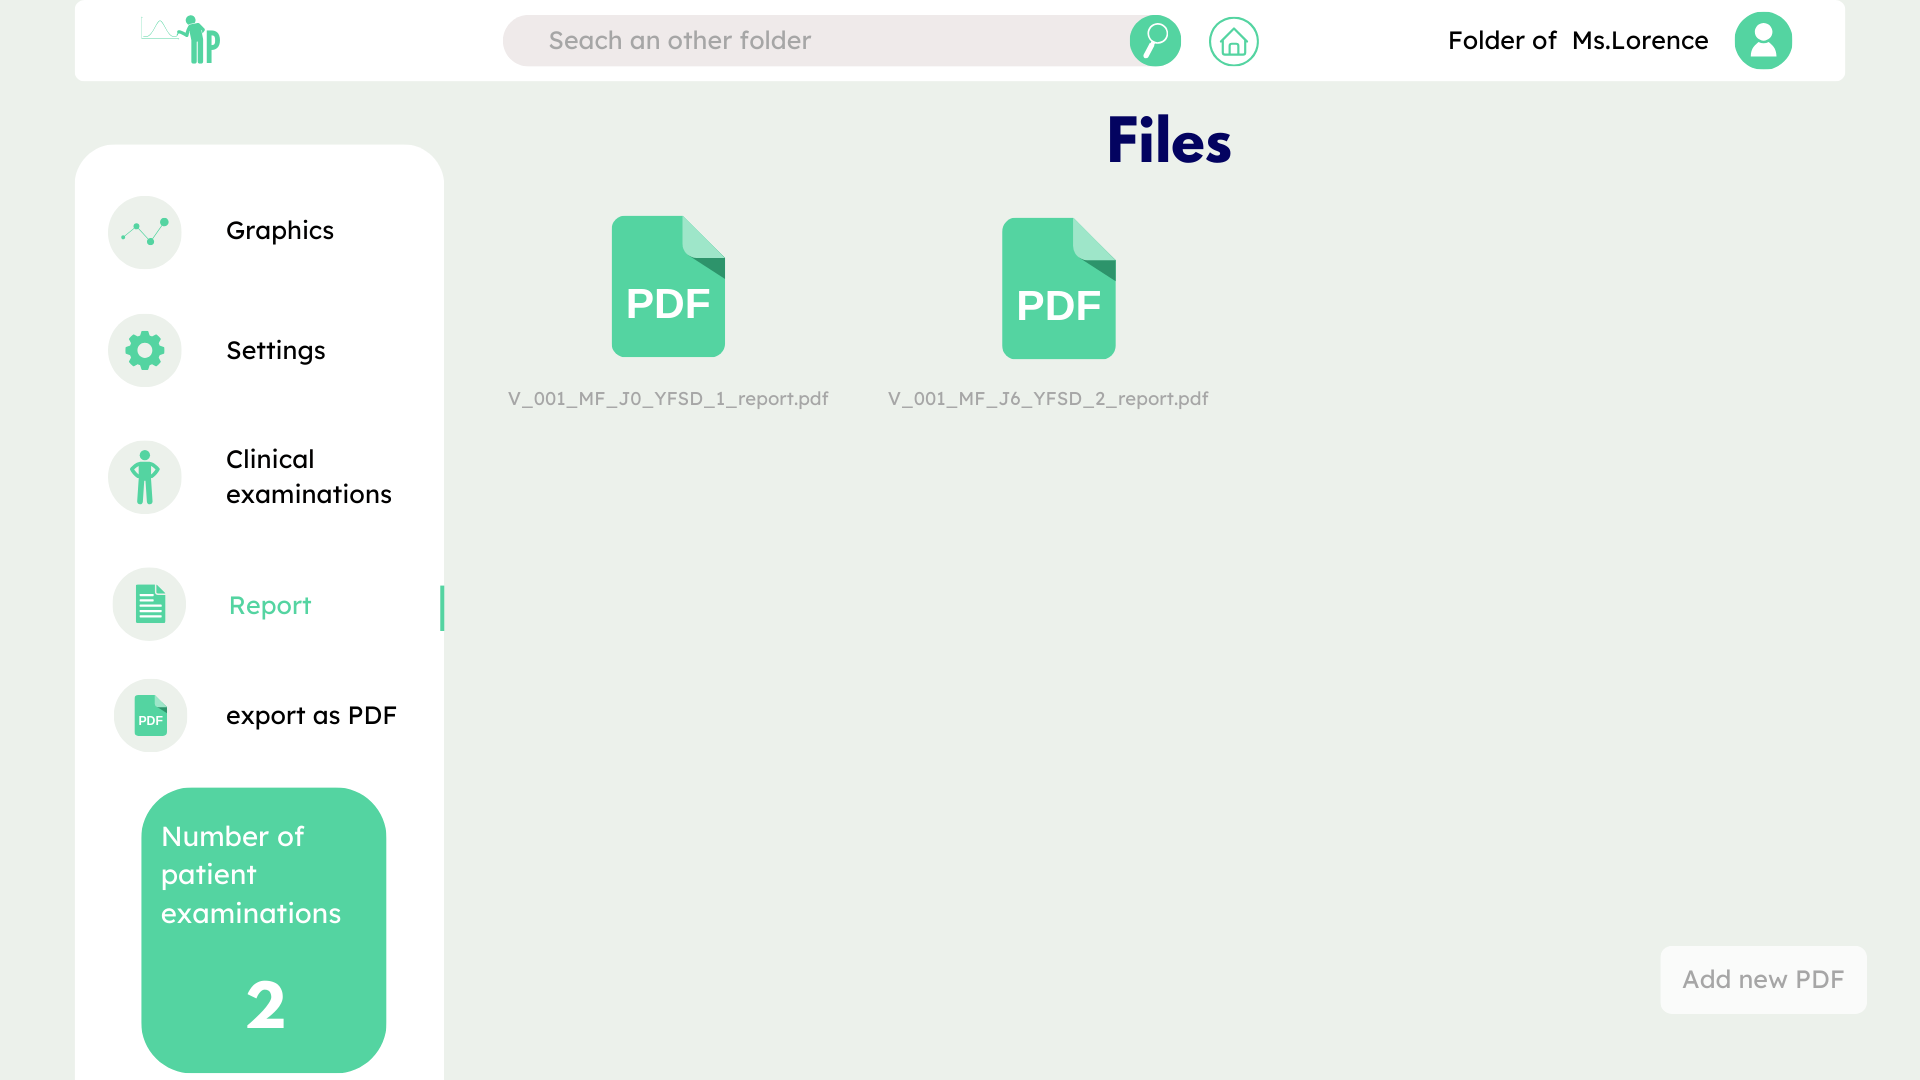
\includegraphics[width=\textwidth]{images/Prototype/15.png}
        \caption*{15}
    \end{minipage}
    \label{fig:plateforme_imaginee}
\end{figure}
